\documentclass{article}

\usepackage{url} 

\usepackage{pdfpages}
\usepackage{lastpage}
\usepackage{fancyhdr}
\usepackage{ngerman}
\usepackage{listings}

\usepackage{tabularx}
\usepackage{subfig}
\usepackage{floatrow}
\usepackage[tableposition=top]{caption}
\floatsetup[table]{capposition=top}



\usepackage{amsmath, amssymb}

\usepackage[utf8]{inputenc}


\usepackage[numbib]{tocbibind}



\newcommand\twodigits[1]{%
   \ifnum#1<10 0#1\else #1\fi
}



\lhead{Abbe-Theorie}
\rhead{13. November 2020\\T. Maier, J. Winkler}
%\cfoot{\twodigits{\thepage}~/ \pageref{LastPage}}
\cfoot{{\thepage}~/ \pageref{LastPage}}

\newcommand{\W}{\text{W}}
\newcommand{\V}{\text{V}}
\newcommand{\A}{\text{A}}


\newcommand{\mini}{\operatorname{min}}


\begin{document}

\parindent0cm


\includepdf{Deckblatt.pdf}


\pagestyle{fancy}

\tableofcontents
\newpage


\section{Aufgabenstellung}

\begin{enumerate}
\item Qualitative  Untersuchung des Zusammenhangs zwischen der  Auflösung  des  Bildes  eines Spaltgitters (Testobjekt) und der Anzahl der transmittierten Beugungsordnungen.
\item Quantitative Bestimmung  des Auflösungsvermögens  einer  Linse  in Abhängigkeit  von  ihrer numerischen Apertur ($N_A$) für zwei unterschiedliche Wellenlängen der Beleuchtung.
\end{enumerate}


\section{Voraussetzungen und Grundlagen}

Die Abbesche Theorie besagt, dass das Auflösungsvermögen eines Objekts maßgeblich durch die Wellenlänge des eingestrahlten Lichts begrenzt wird. Das Auflösungsvermögen ist dabei die Fähigkeit eines Instruments Objektdetails noch getrennt abbilden zu können. Eine der Grundlage für diese Theorie bildet das Huygenssche Prinzip, wonach jeder Punkt einer Wellenfront der Ausgangspunkt einer neuen kugelförmigen Elementarwelle ist.

Licht trifft also auf ein Gitter, es bilden sich kugelförmige Wellen und es kann sowohl konstruktive als auch destruktive Interferenz beobachtet werden. Die Abbesche Theorie sagt hier, dass jedoch mindestens die Maxima nullter und erster Ordnung von einer Linse erfasst werden müssen, um überhaupt eine Auflösung zu erhalten. Außerdem kann die Linse (rein technisch) nicht unendlich groß gebaut (d.h. es können nie alle Maxima erfasst werden) und auch nicht beliebig nahe an das Gitter herangebracht werden. Der Zusammenhang zwischen Einfallswinkel $\alpha$ des Lichts, das höchstens von der Linse erfasst werden kann und Brechzahl $n$ des Mediums, in dem sich die Apertur befindet, ist durch die sogenannte numerische Apertur $N_A$ (Auflösungvermögen des Mikroskops) gegeben
\begin{align}
N_A = n\cdot\sin(\alpha)
\end{align}
Betrachtet man nun zwei Punkte eines Gitters, die im Abstand $d$ voneinander entfernt sind und ebenfalls jeweils eine kugelförmige Welle aussenden, so ergibt sich der Zusammenhang
\begin{align}
d \ge \frac{\lambda}{\sin(\alpha)\cdot n}
\end{align}
bzw. durch Einsetzen
\begin{align}
d \ge \frac{\lambda}{N_A} 
\end{align}
$\alpha$ entspricht in diesen Formeln dem Winkel zwischen nullter und erster Ordnung der Maxima und $\lambda$ entspricht der Wellenlänge des eingestrahlten Lichts.


Der kleinstmögliche Abstand $d_{\operatorname{min}}$ ist dann gegeben durch
\begin{align}
\label{eq:theor_aufl}
d_{\text{min}} = 0.61 \cdot \frac{\lambda}{N_A}
\end{align}
Außerdem kann für $r<<f$ und $n=1$ (also Luft bzw Vakuum) angenommen werden, dass
\begin{align}
\label{eq:na}
N_A \approx r/f
\end{align}
wobei $f$ der Abstand zwischen Linse und Blende und $r$ der Radius der Lochblende ist.  (vgl. \cite{quelle1} \cite{quelle2} \cite{quelle3})

Zum ähnlichen Überlegungen kommt man aufgrund des Rayleigh-Kriteriums zur optischen Mikroskopie, welches besagt, dass zwei Punkte im Abstand $x$ gerade dann noch auflösbar sind, wenn das Beugungsscheibchen des ersten Objekts auf das erste Minimum des Beugungsscheibchens des zweiten Objekts fällt. (vgl. \cite{quelle4} \cite{quelle5})
\begin{align}
x = \frac{\frac{1.22}{2}\cdot \lambda}{N_A}
\end{align}



\begin{figure}[H]
\caption{Intensitätsverteilung bei einem Beugungsgitter mit 8 Spalten. Quelle: \cite{demtroeder}}
\label{fig:beugung}
{\centering
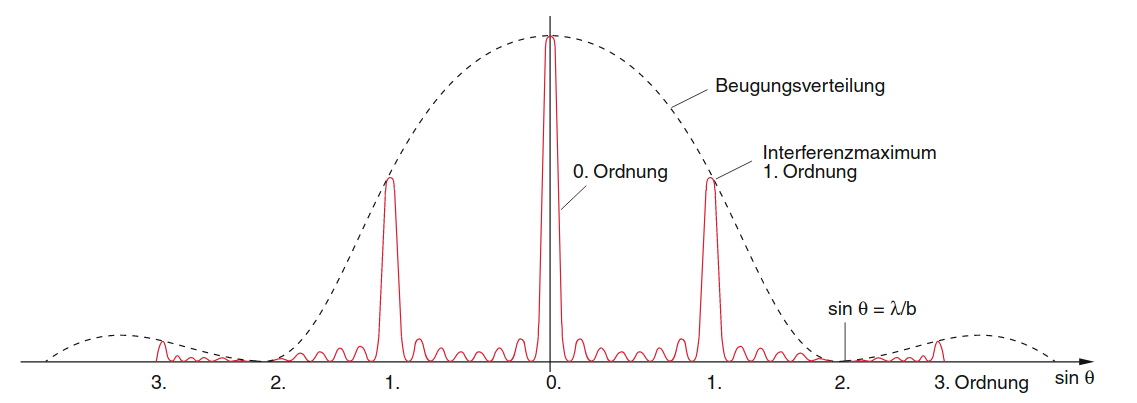
\includegraphics[scale=0.9]{demtr_10_44.png}
~
}
\end{figure}





\section{Geräteliste}

\begin{table}[H]
\caption{Liste der verwendeten Geräte}

~

\begin{tabular}{l|p{3cm}p{3cm}llll}
Abk. & Bezeichnung  & Typ & Gerätenummer & Unsicherheit \\
\hline
LA & Diodenge\-pumpter Festkörperlaser THOR-Labs  & Festkörperlaser $\lambda~=~531.9~$nm & LDS5 & $\Delta \lambda = 0.05~$nm \\
\hline
BL & Blaue LED &  $\lambda=470~$nm & & $\Delta \lambda = 5~$nm \\
\hline
RL & Rote LED &  $\lambda=635~$nm & & $\Delta \lambda = 5~$nm \\
\hline
TO & Testobjekt & 1951 USAF Target  \\
\hline
L1 & Linse 1 & $f_1 = 200~$mm & & $\Delta f_1 = 1~$mm \\
\hline
L2 & Abbildungslinse 2 & $f_2= 60~$mm & & $\Delta f_2 = 1~$mm\\
\hline
L3 & Hilfslinse & $f_3 = 50~$mm, klappbar & & $\Delta f_3 = 1~$mm \\
\hline
B & Lochblenden und Irisblende & $d_1=2~$mm ~ ~ ~ ~ $d_2=3~$mm   ~~~~~~~~~~~~ $d_3=6~$mm & &  $\Delta d = 0.1~$mm \\
\hline
F & Filterrad für LEDs & \\
\hline
K & Kamera & & DMK42AUC03
\end{tabular}

\end{table}



\section{Beschreibung der Versuchsanordnung}


\begin{figure}[H]
\caption{Das verwendete Testobjekt, USAF 1951. aus \cite{quelle6}}
\label{fig:usaf}
{\centering
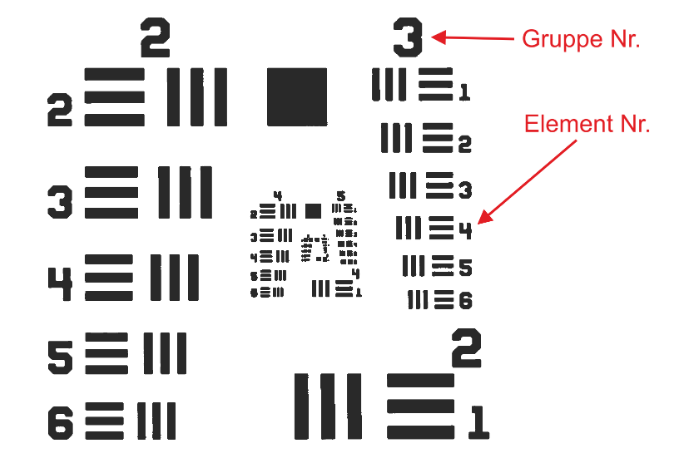
\includegraphics[scale=1.5]{usaf.png}
~
}
\end{figure}


Als darzustellendes Objekt wird Grafik \ref{fig:usaf} verwendet. Diese dient zur Bestimmung des Auflösevermögens von optischen Geräten. Es gibt mehrere Gruppen, die jeweils 6 Elemente haben. Ein Element besteht jeweils aus 3 horizontalen und 3 vertikalen Linien. Die Auflösung kann dadurch bestimmt werden, dass man die entsprechende Gruppe und das entsprechende Element angibt, mit einem / getrennt. Das Auflösevermögen wird durch jenes Element (bzw. Gruppe) bestimmt, dass am kleinsten ist und wo man trotzdem noch die horizontalen von den vertikalen Linien unterscheiden kann. Das Auflösevermögen kann in Tabelle \ref{tab:aufl} abgelesen werden.




\begin{table}[H]
\caption{Auflösungsvermögen je nach nach Element und Gruppe mit der Einheit mm$^{-1}$. Entnommen aus \cite{quelle6}. Die Werte stellen die räumliche Frequenz in der Einheit 1/mm dar.}
\label{tab:aufl}
\begin{tabular}{|l||l|l|l|l|l|l|l|l|l|l|l|}
\hline
\textbf{Elem. Nr.} & \multicolumn{10}{|c|}{\textbf{Gruppen Nr.}}\\
\hline
& -2 & -1 & 0 & 1 & 2 & 3 & 4 & 5 & 6 & 7 \\
\hline
1 & 0.250 & 0.500 & 1.00 & 2.00 & 4.00 & 8.00 & 16.00 & 32.0 & 64.0 & 128.0 \\
\hline
2 & 0.280 & 0.561 & 1.12 & 2.24 & 4.49 & 8.98 & 17.95 & 36.0 & 71.8 & 144.0 \\
\hline
3 & 0.315 & 0.630 & 1.26 & 2.52 & 5.04 & 10.10 & 20.16 & 40.3 & 80.6 &  161.0 \\
\hline
4 & 0.353 & 0.707 & 1.41 & 2.83 & 5.66 & 11.30 & 22.62 & 45.3 & 90.5 & 181.0 \\
\hline
5 & 0.397 & 0.793 & 1.59 & 3.17 & 6.35 & 12.70 & 25.39 & 50.8 & 102.0 & 203.0 \\
\hline
6 & 0.445 & 0.891 & 1.78 & 3.56 & 7.13 & 14.30 & 28.50 & 57.0 & 114.0 & 228.0 \\
\hline
\end{tabular}
\end{table}






\begin{figure}[H]
\caption{Aufbau (inkl. Abmessungen) des Versuchs; $L_1$: $f_1= 200~$mm, $F$: Filterrad mit 2 LEDs, Graufilter und freiem Durchgang, $T$: Testobjekt; $L_2$: $f_2= 60~$mm; $B$: Filterrad mit 3 Lochblenden, einer Irisblende und einer Drahtblende, $L_3$ (einklappbar): $f_3= 50~$mm. Quelle: \cite{quelle6}}
\label{fig:aufbau}
{\centering
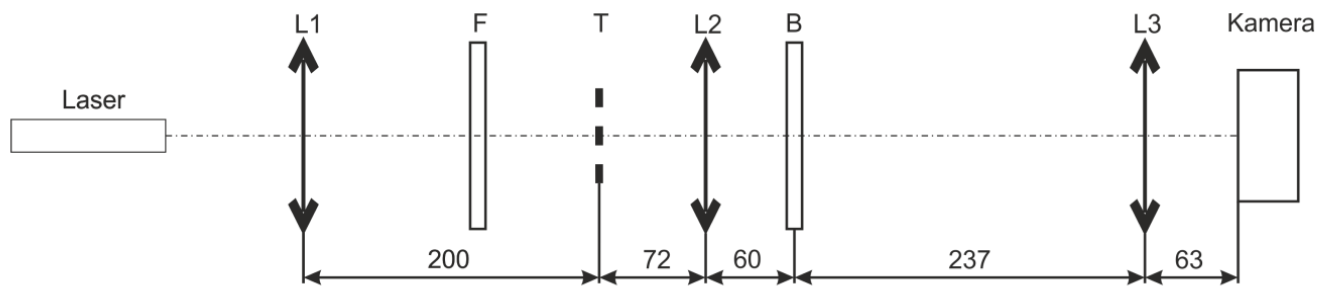
\includegraphics[scale=1]{versuch.png}
~
}
\end{figure}








\section{Versuchsdurchführung und Messwerte}

\subsection{Beugungsordnungen und Auflösung}

Es soll der Zusammenhang zwischen Beugungsordnungen und Auflösung gezeigt werden. 

Zuerst wurde die geöffnete Irisblende am Filterrand $B$ in den Strahlengang gedreht und die Linse $L_3$ aus dem Strahlengang rausgeklappt. Dann wurde das Objekt scharfgestellt, indem es mit einer roten LED-Lampe beleuchtet wurde. Danach wurden die drei vertikalen Balken des 3/4 gesucht und zentriert. Anschließend wurde noch die LED-Beleuchtung durch eine Laserbeleuchtung ersetzt und das Bild des Objektes, sowie das zugehörige Beugungsbild aufgenommen.

Mit Hilfe der Irisblende kann die Anzahl der Beugungsordnungen reduziert werden.

Die Aufnahmen von Tanja Maier sind hier als Abbildungen~\ref{fig:bbild_0_tm} bis \ref{fig:bild_voll_tm} aufgelistet.
Die Aufnahmen von Johannes Winkler wurden wegen COVID-19 durch die zur Verfügung gestellten Aufnahmen ersetzt. Diese sind als Abbildungen~\ref{fig:bbild_0_jw} bis \ref{fig:bild_voll_jw} aufgelistet.

\subsubsection{Bilder aufgenommen von Tanja Maier}
 
\begin{minipage}[t]{.45\textwidth}
\begin{figure}[H]
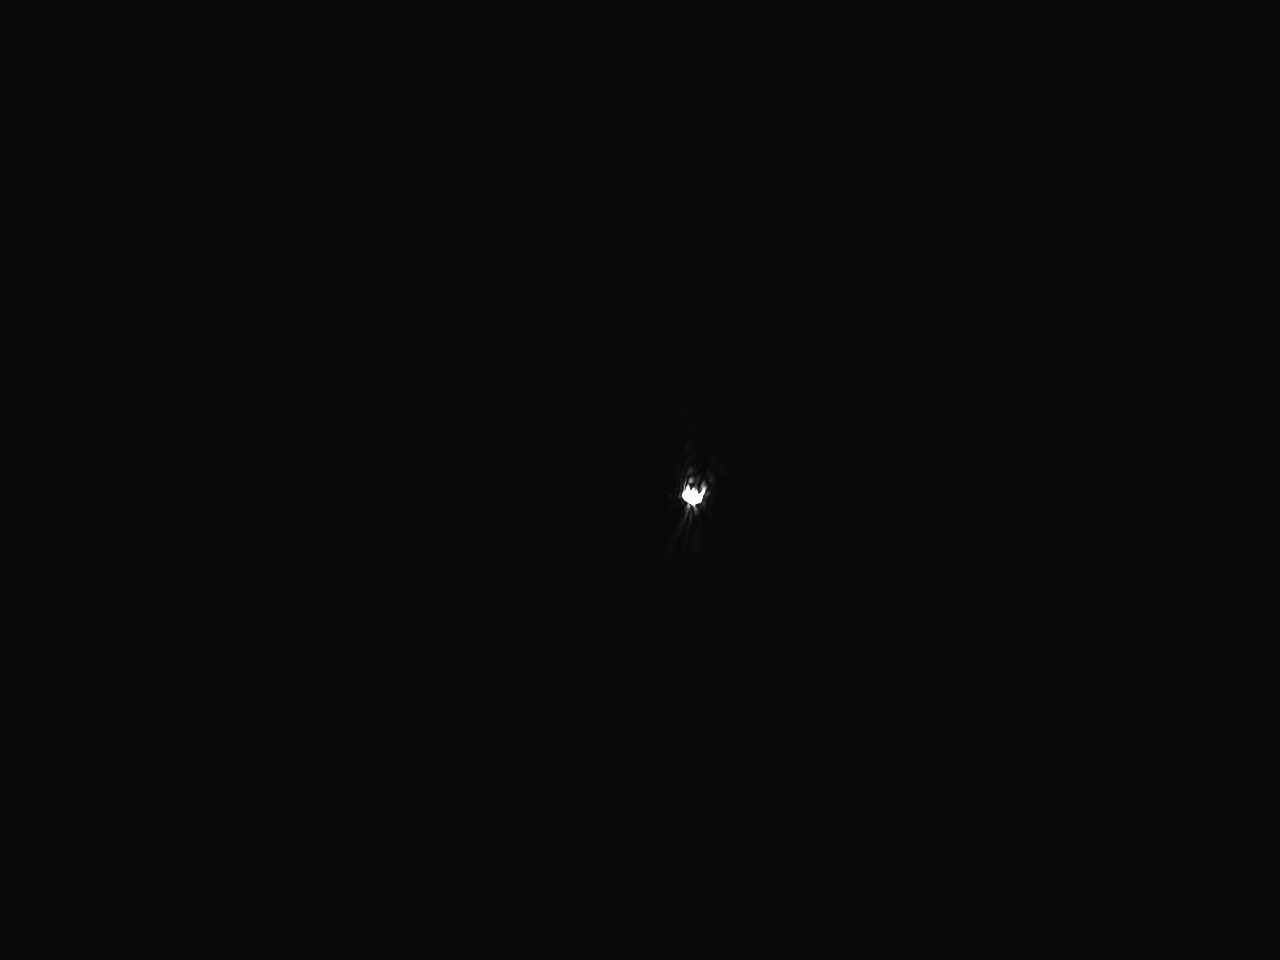
\includegraphics[scale=0.1]{tm/Beugungsbild_0.jpg}
\caption{Aufnahme des Beugungsbildes 0. Ordnung.}
\label{fig:bbild_0_tm}
\end{figure}
\end{minipage}
\hfill
\noindent
\begin{minipage}[t]{.45\textwidth}
\begin{figure}[H]

\includegraphics[scale=0.1]{tm/Bild_0.jpg}
\caption{Aufnahme des Bildes 0. Ordnung.}
\label{fig:bild_0_tm}
\end{figure}
\end{minipage}

\begin{minipage}[t]{.45\textwidth}
\begin{figure}[H]
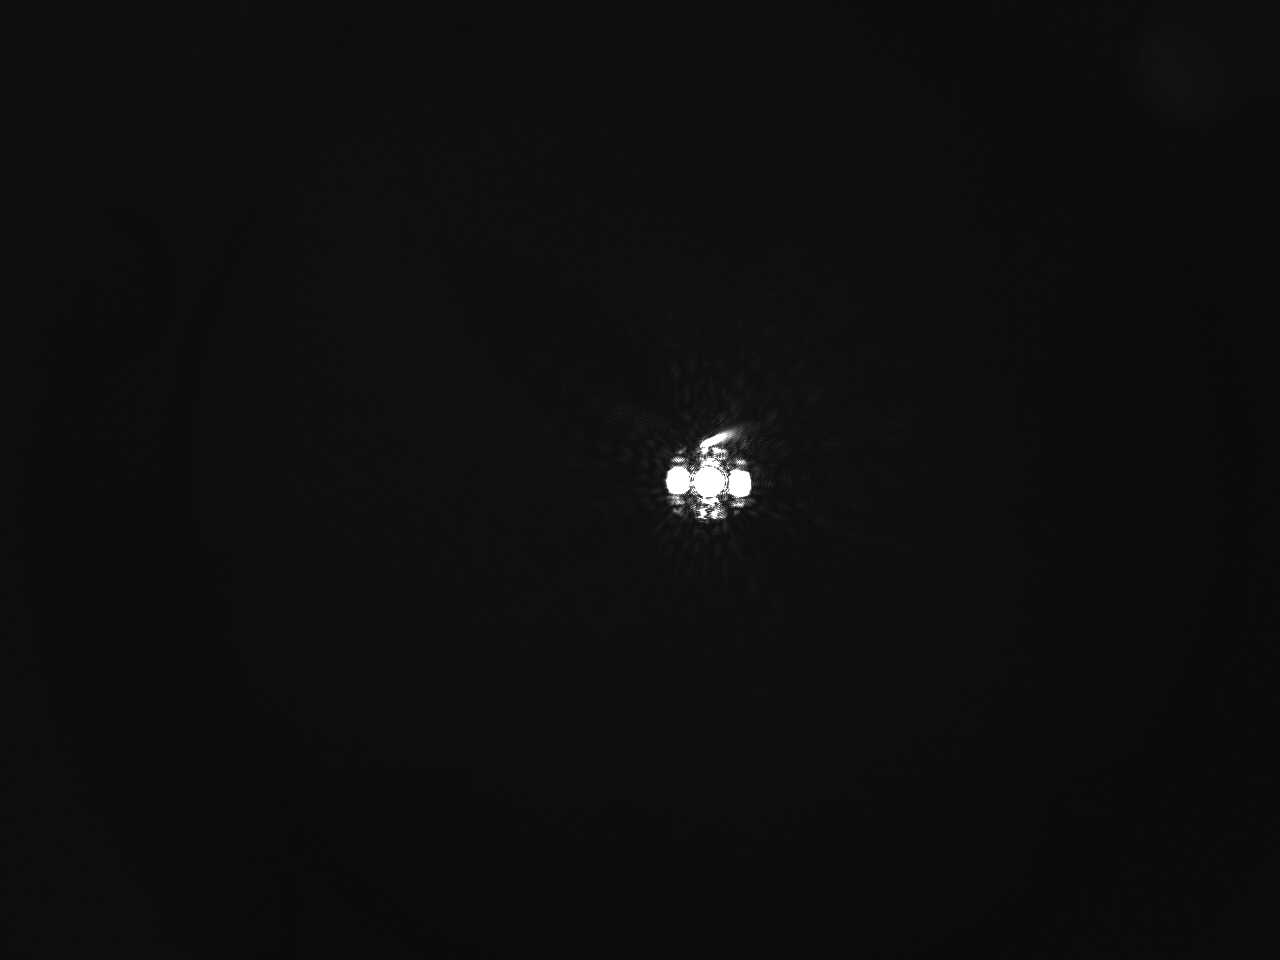
\includegraphics[scale=0.1]{tm/Beugungsbild_1.jpg}
\caption{Aufnahme des Beugungsbildes 1. Ordnung.}
\label{fig:bbild_1_tm}
\end{figure}
\end{minipage}
\hfill
\noindent
\begin{minipage}[t]{.45\textwidth}
\begin{figure}[H]

\includegraphics[scale=0.1]{tm/Bild_1.jpg}
\caption{Aufnahme des Bildes 1. Ordnung.}
\label{fig:bild_1_tm}
\end{figure}
\end{minipage}



\begin{minipage}[t]{.45\textwidth}
\begin{figure}[H]
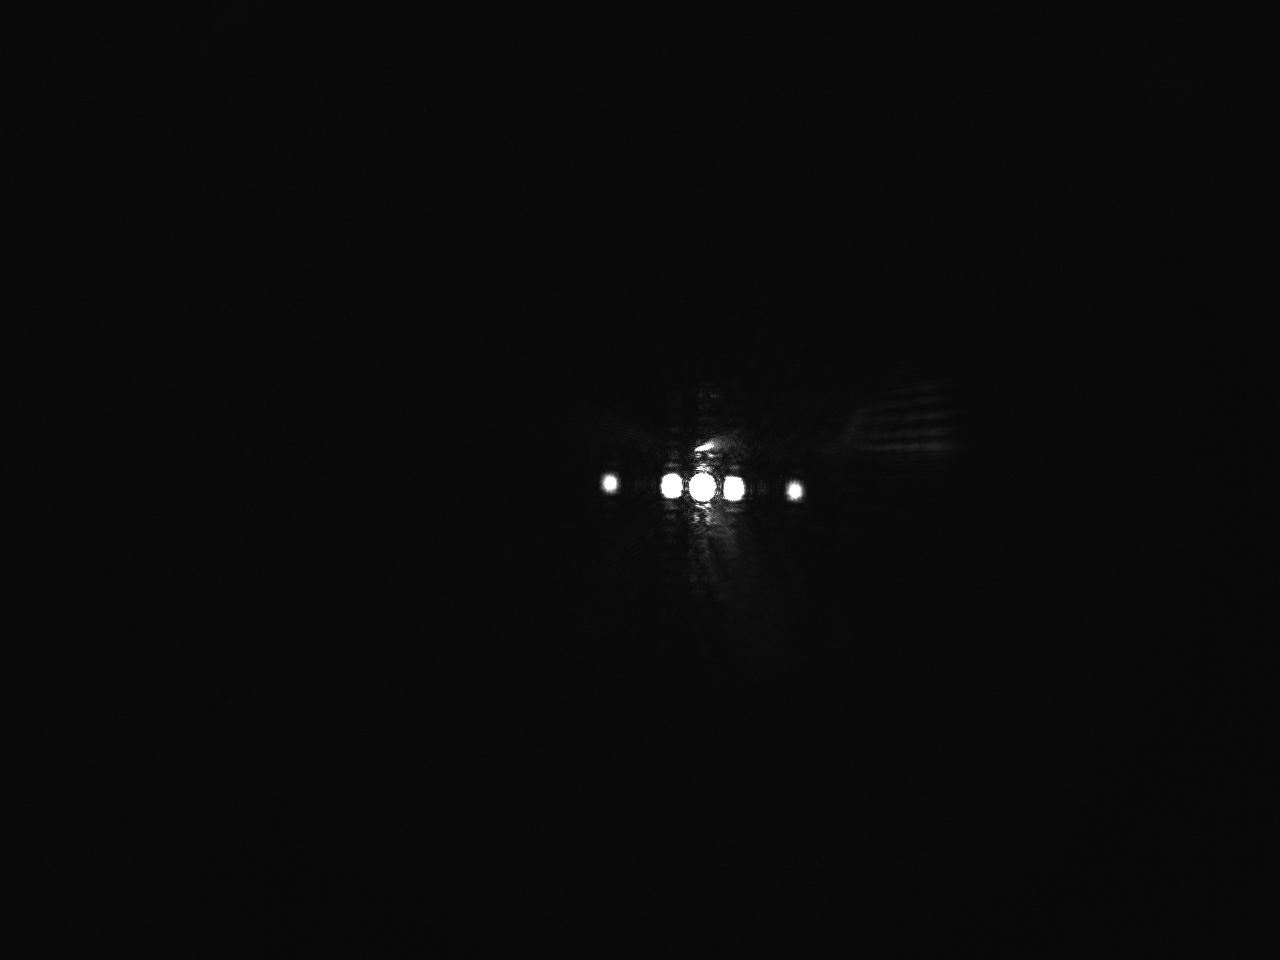
\includegraphics[scale=0.1]{tm/Beugungsbild_3.jpg}
\caption{Aufnahme des Beugungsbildes 3. Ordnung.}
\label{fig:bbild_3_tm}
\end{figure}
\end{minipage}
\hfill
\noindent
\begin{minipage}[t]{.45\textwidth}
\begin{figure}[H]
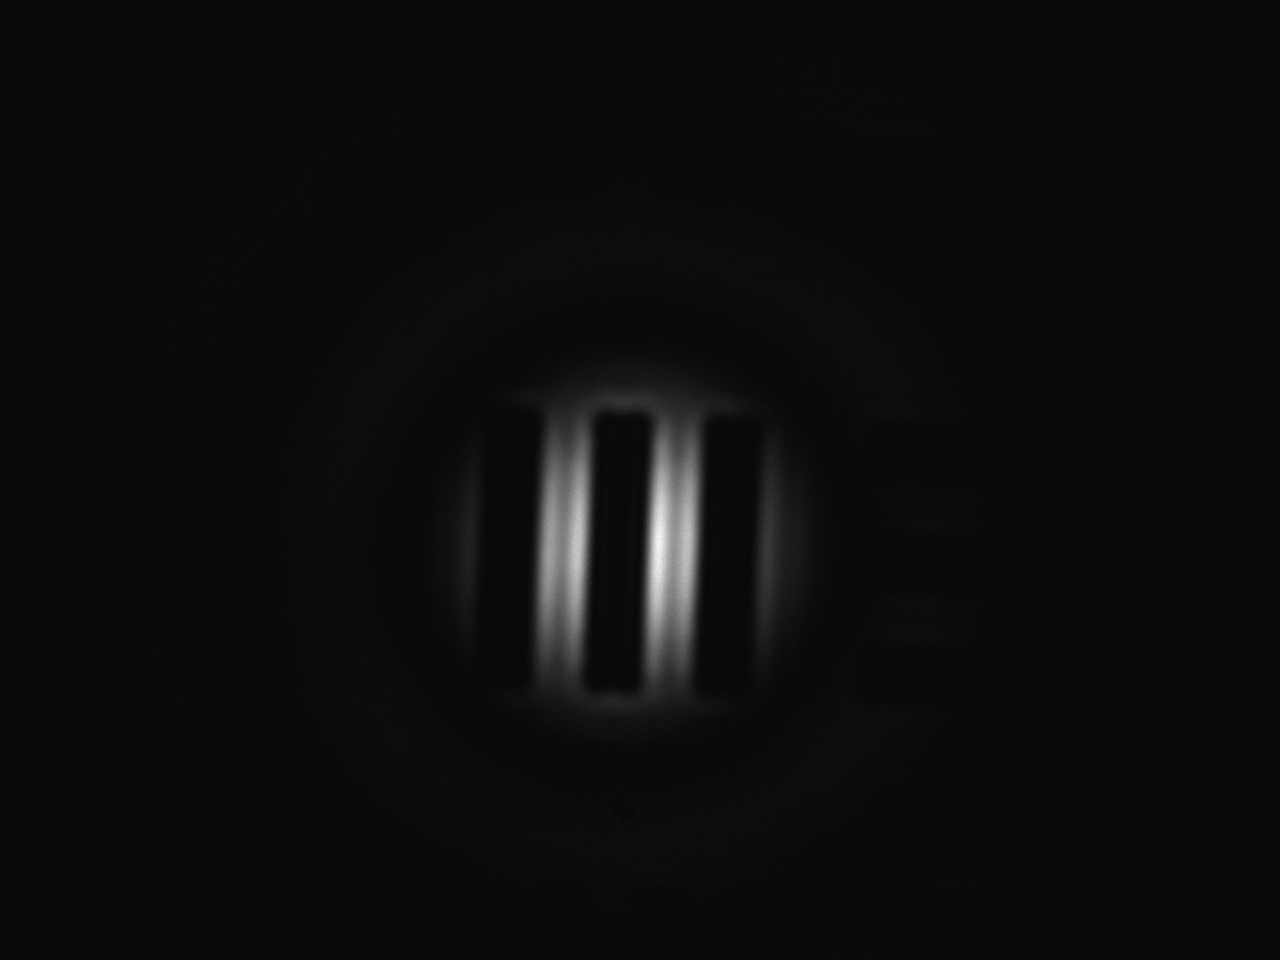
\includegraphics[scale=0.1]{tm/Bild_3.jpg}
\caption{Aufnahme des Bildes 3. Ordnung.}
\label{fig:bild_3_tm}
\end{figure}
\end{minipage}






\begin{minipage}[t]{.45\textwidth}
\begin{figure}[H]

\includegraphics[scale=0.1]{tm/Beugungsbild_5.jpg}
\caption{Aufnahme des Beugungsbildes 5. Ordnung.}
\label{fig:bbild_5_tm}
\end{figure}
\end{minipage}
\hfill
\noindent
\begin{minipage}[t]{.45\textwidth}
\begin{figure}[H]

\includegraphics[scale=0.1]{tm/Bild_5.jpg}
\caption{Aufnahme des Bildes 5. Ordnung.}
\label{fig:bild_5_tm}
\end{figure}
\end{minipage}




\begin{minipage}[t]{.45\textwidth}
\begin{figure}[H]
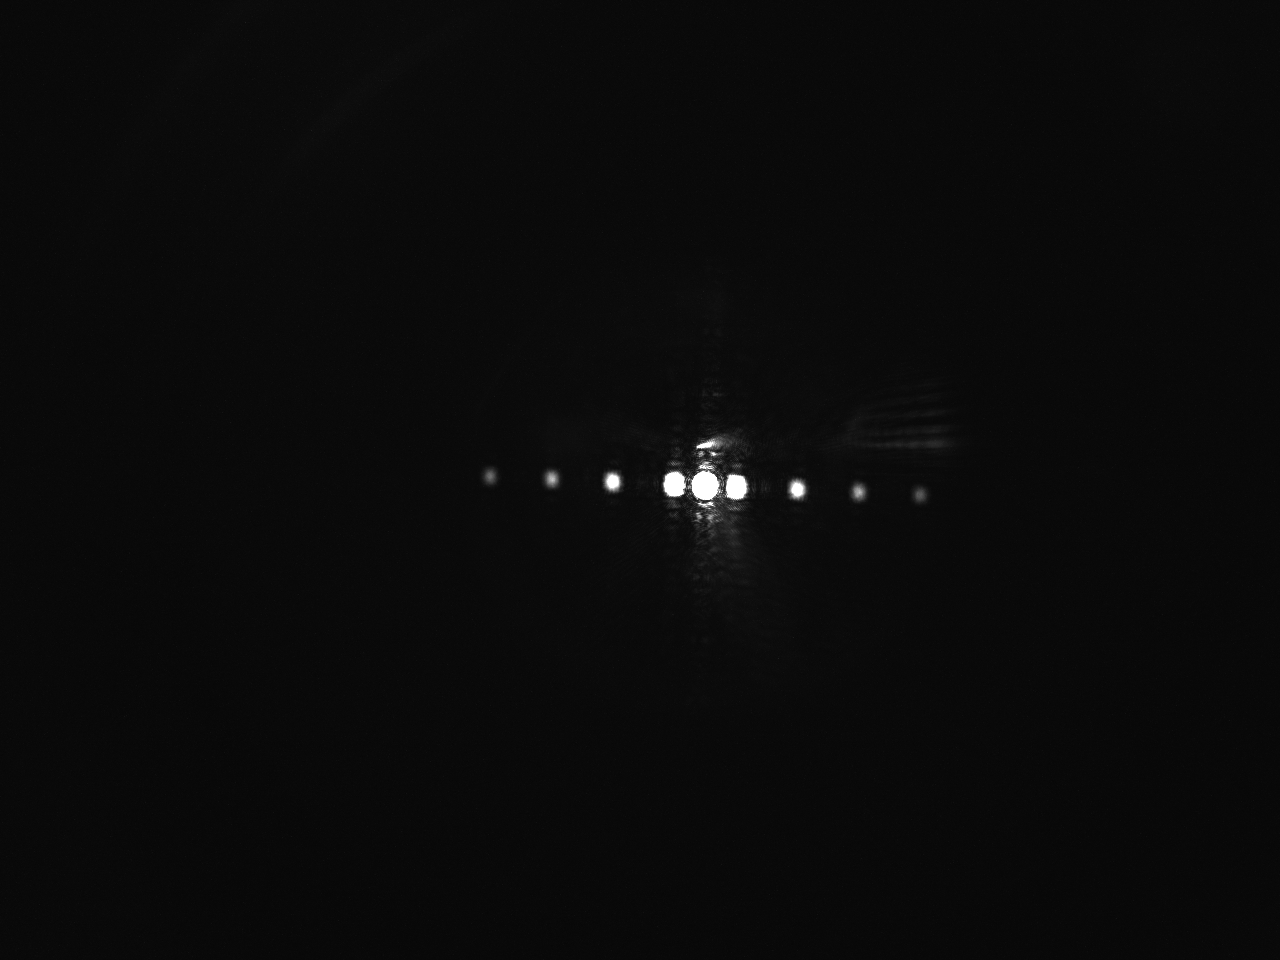
\includegraphics[scale=0.1]{tm/Beugungsbild_7.jpg}
\caption{Aufnahme des Beugungsbildes 7. Ordnung.}
\label{fig:bbild_7_tm}
\end{figure}
\end{minipage}
\hfill
\noindent
\begin{minipage}[t]{.45\textwidth}
\begin{figure}[H]

\includegraphics[scale=0.1]{tm/Bild_7.jpg}
\caption{Aufnahme des Bildes 7. Ordnung.}
\label{fig:bild_7_tm}
\end{figure}
\end{minipage}



\begin{minipage}[t]{.45\textwidth}
\begin{figure}[H]
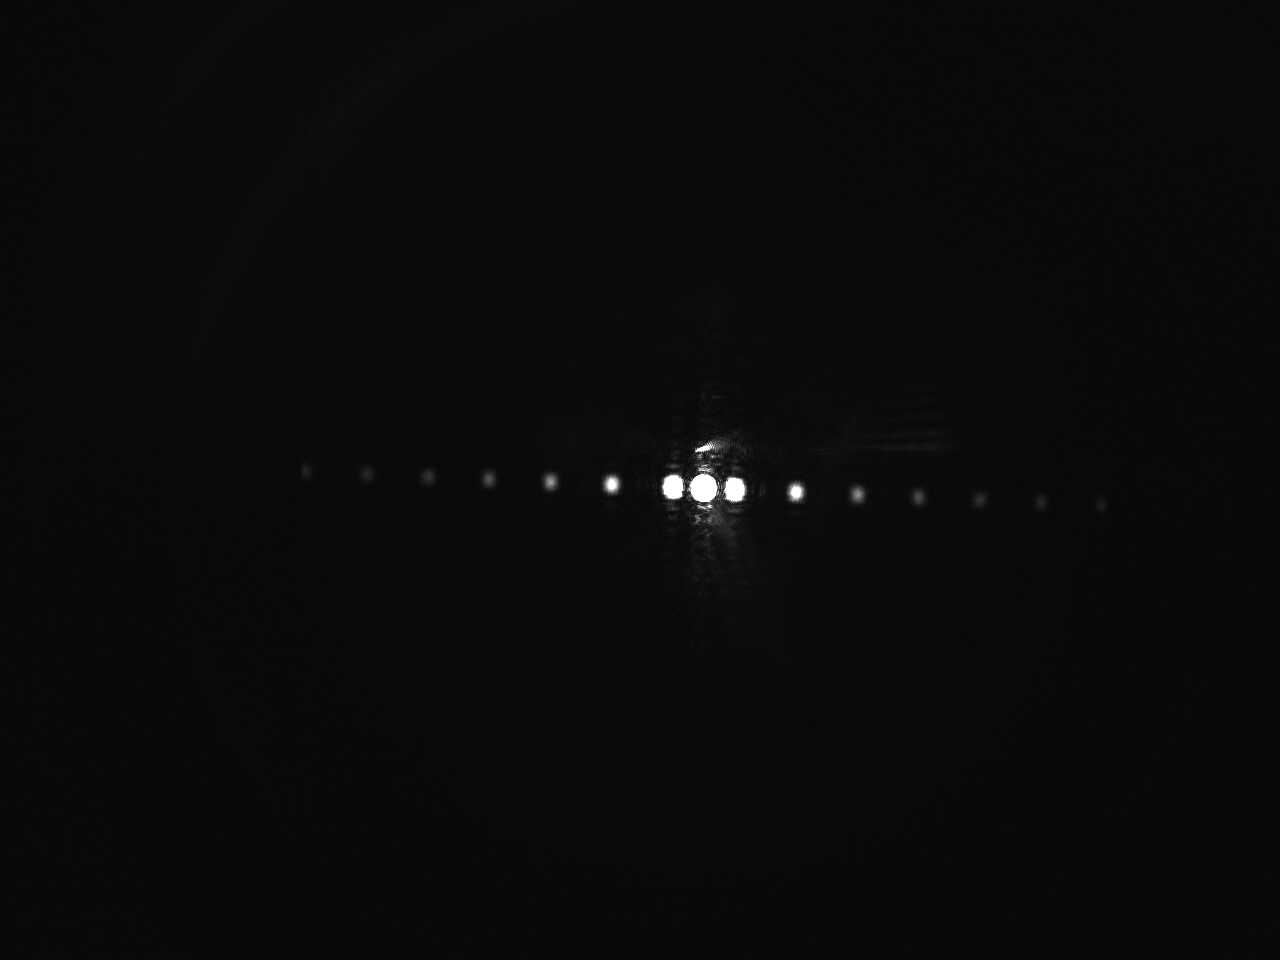
\includegraphics[scale=0.1]{tm/Beugungsbild_voll.jpg}
\caption{Aufnahme des Beugungsbildes mit vollständig offener Irisblende.}
\label{fig:bbild_voll_tm}
\end{figure}
\end{minipage}
\hfill
\noindent
\begin{minipage}[t]{.45\textwidth}
\begin{figure}[H]

\includegraphics[scale=0.1]{tm/Bild_voll.jpg}
\caption{Aufnahme des Bildes 7. Ordnung mit vollständig offener Irisblende.}\label{fig:bild_voll_tm}
\end{figure}
\end{minipage}











\subsubsection{Bilder aus Mitschrift von Moodle entnommen}




\begin{minipage}[t]{.45\textwidth}
\begin{figure}[H]
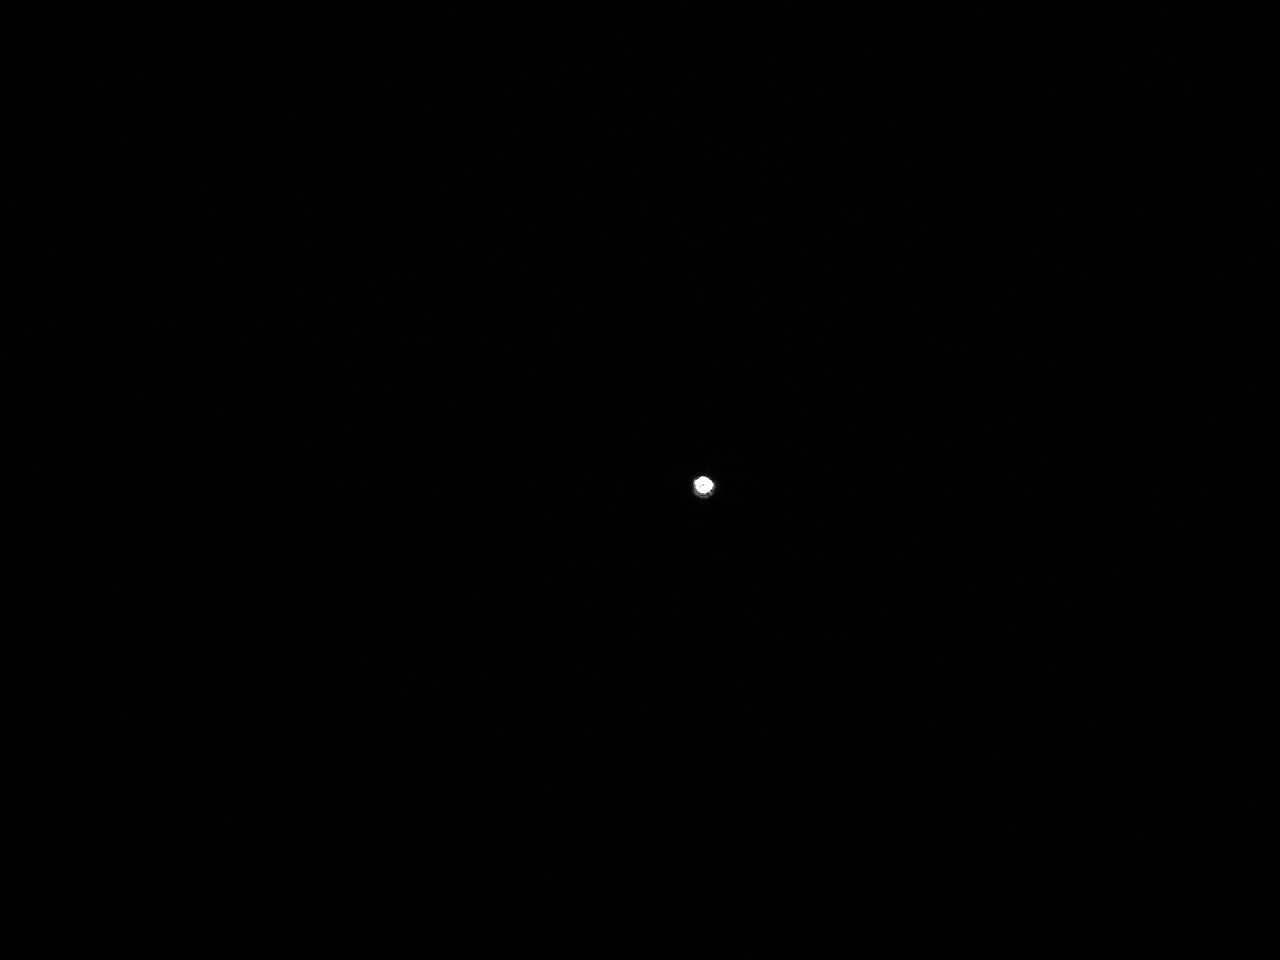
\includegraphics[scale=0.1]{jw/L_BB_5.jpg}
\caption{Aufnahme des Beugungsbildes 0. Ordnung. Aufnahme wurde zur Verfügung gestellt.}
\label{fig:bbild_0_jw}
\end{figure}
\end{minipage}
\hfill
\noindent
\begin{minipage}[t]{.45\textwidth}
\begin{figure}[H]
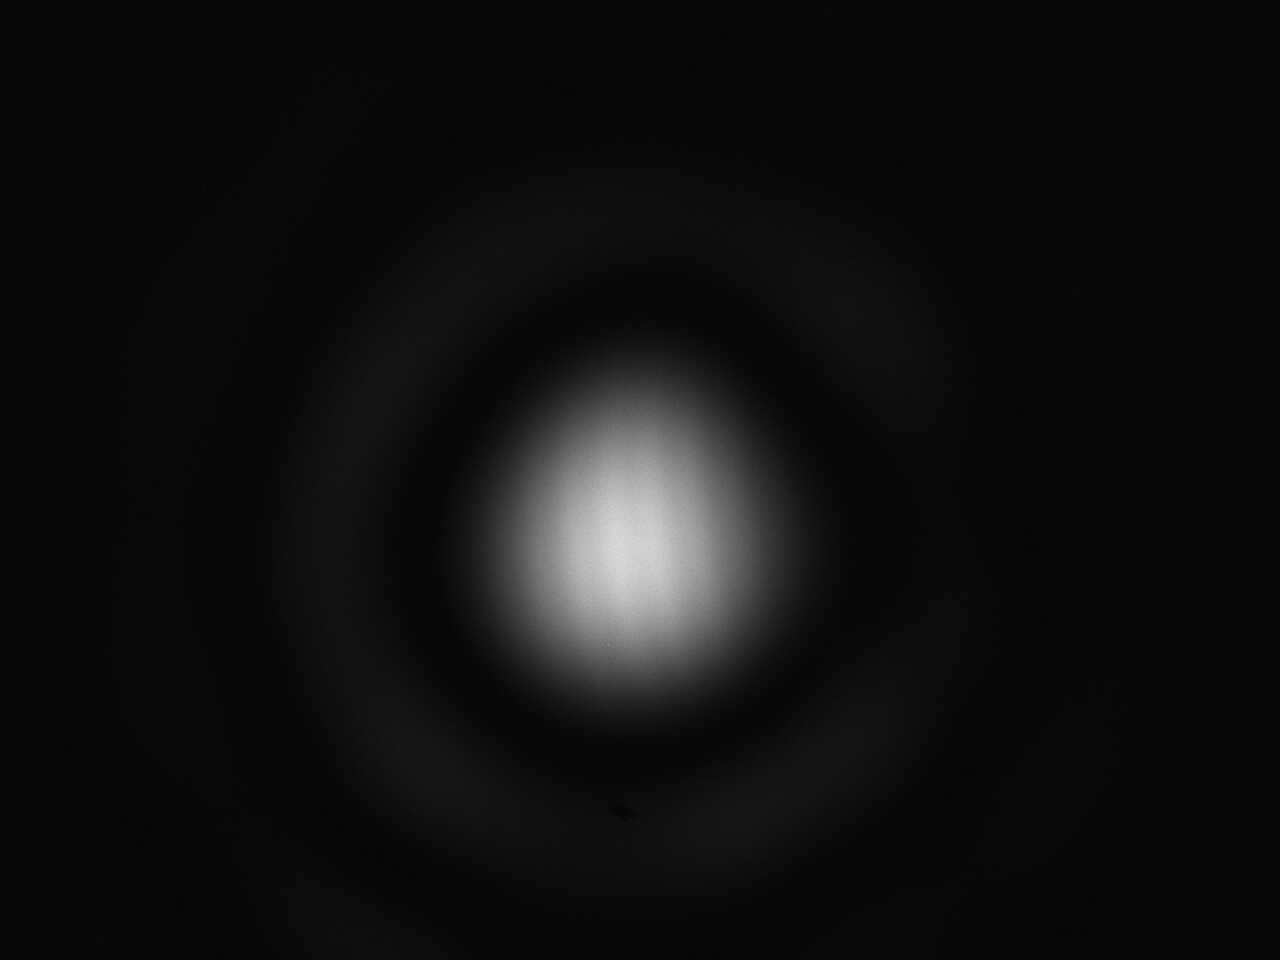
\includegraphics[scale=0.1]{jw/L_OB_5.jpg}
\caption{Aufnahme des Bildes 0. Ordnung. Aufnahme wurde zur Verfügung gestellt.}\label{fig:bild_0_jw}
\end{figure}
\end{minipage}

\begin{minipage}[t]{.45\textwidth}
\begin{figure}[H]
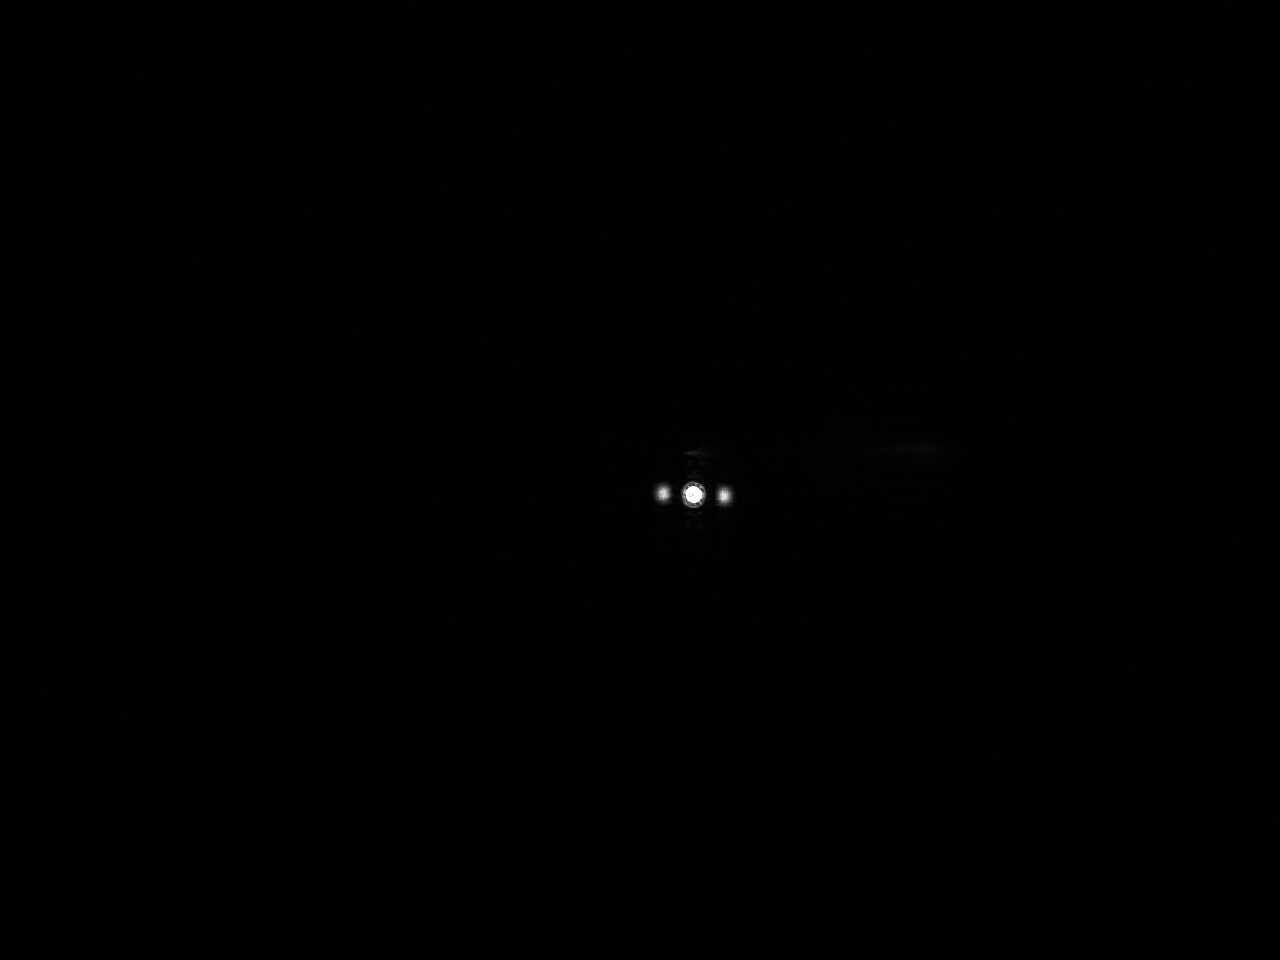
\includegraphics[scale=0.1]{jw/L_BB_4.jpg}
\caption{Aufnahme des Beugungsbildes 1. Ordnung. Aufnahme wurde zur Verfügung gestellt.}
\label{fig:bbild_1_jw}
\end{figure}
\end{minipage}
\hfill
\noindent
\begin{minipage}[t]{.45\textwidth}
\begin{figure}[H]
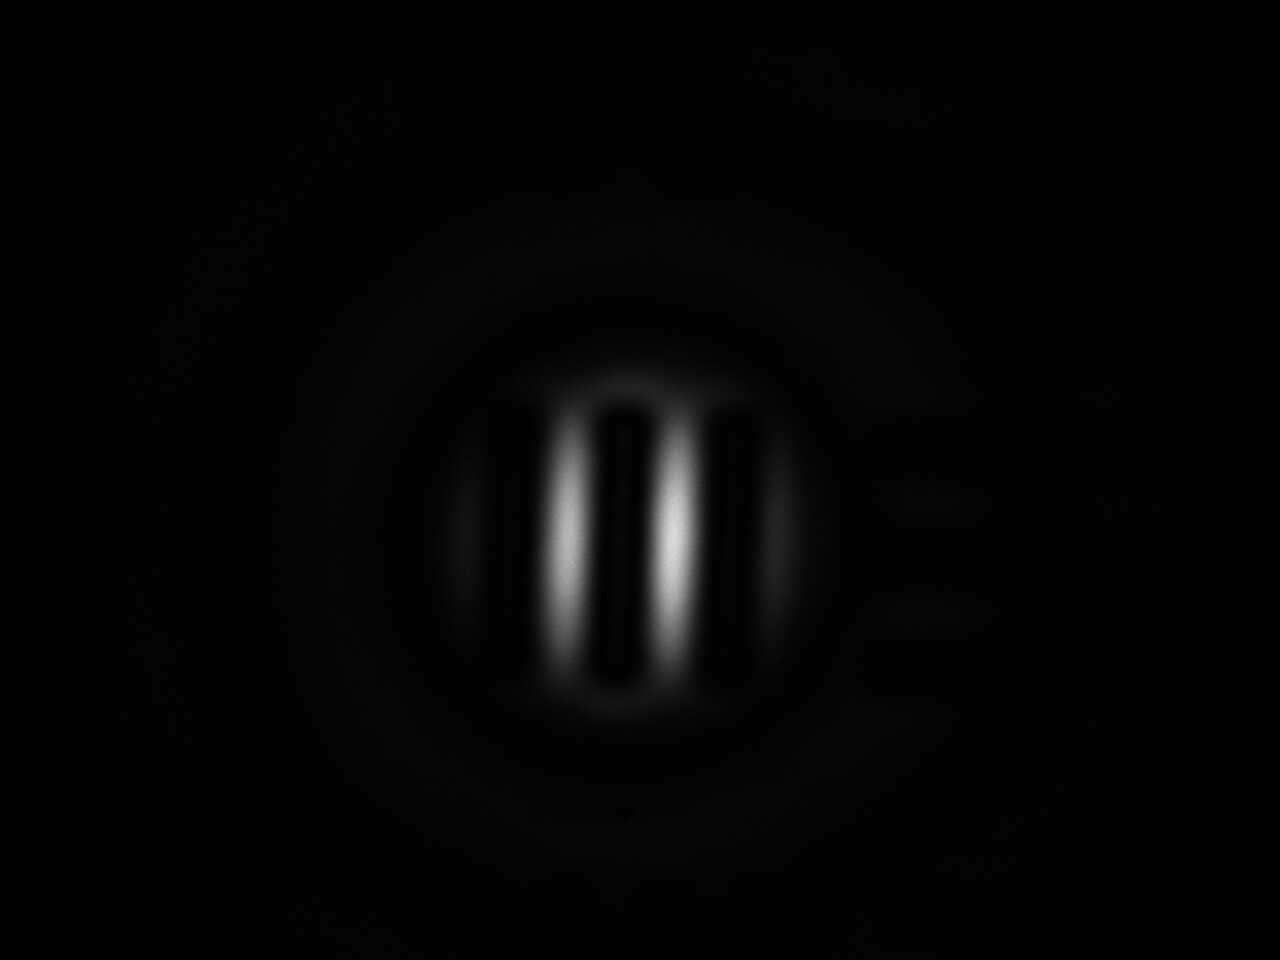
\includegraphics[scale=0.1]{jw/L_OB_4.jpg}
\caption{Aufnahme des Bildes 1. Ordnung. Aufnahme wurde zur Verfügung gestellt.}\label{fig:bild_1_jw}
\end{figure}
\end{minipage}



\begin{minipage}[t]{.45\textwidth}
\begin{figure}[H]
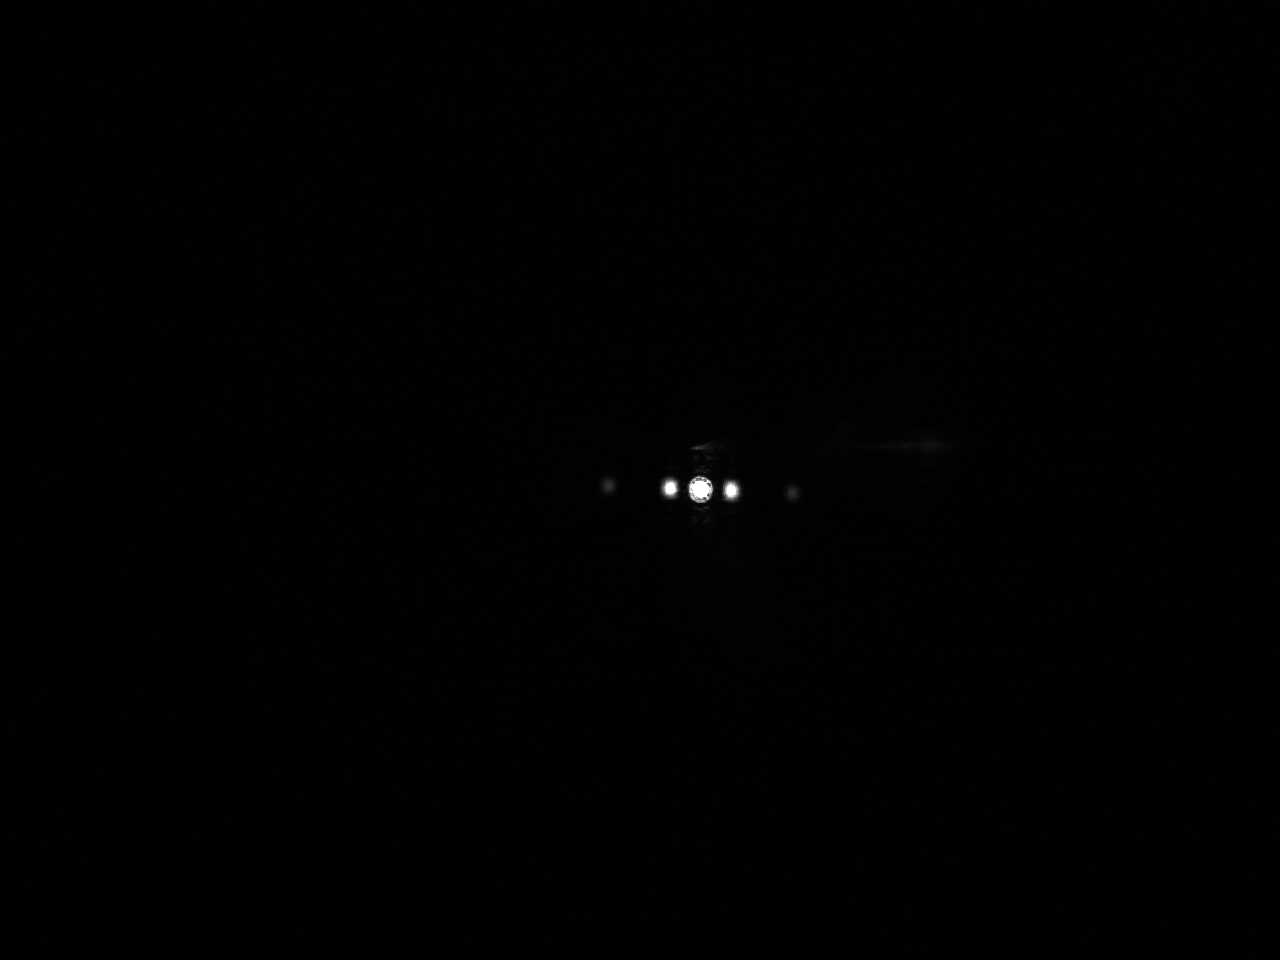
\includegraphics[scale=0.1]{jw/L_BB_3.jpg}
\caption{Aufnahme des Beugungsbildes 3. Ordnung. Aufnahme wurde zur Verfügung gestellt.}
\label{fig:bbild_3_jw}
\end{figure}
\end{minipage}
\hfill
\noindent
\begin{minipage}[t]{.45\textwidth}
\begin{figure}[H]
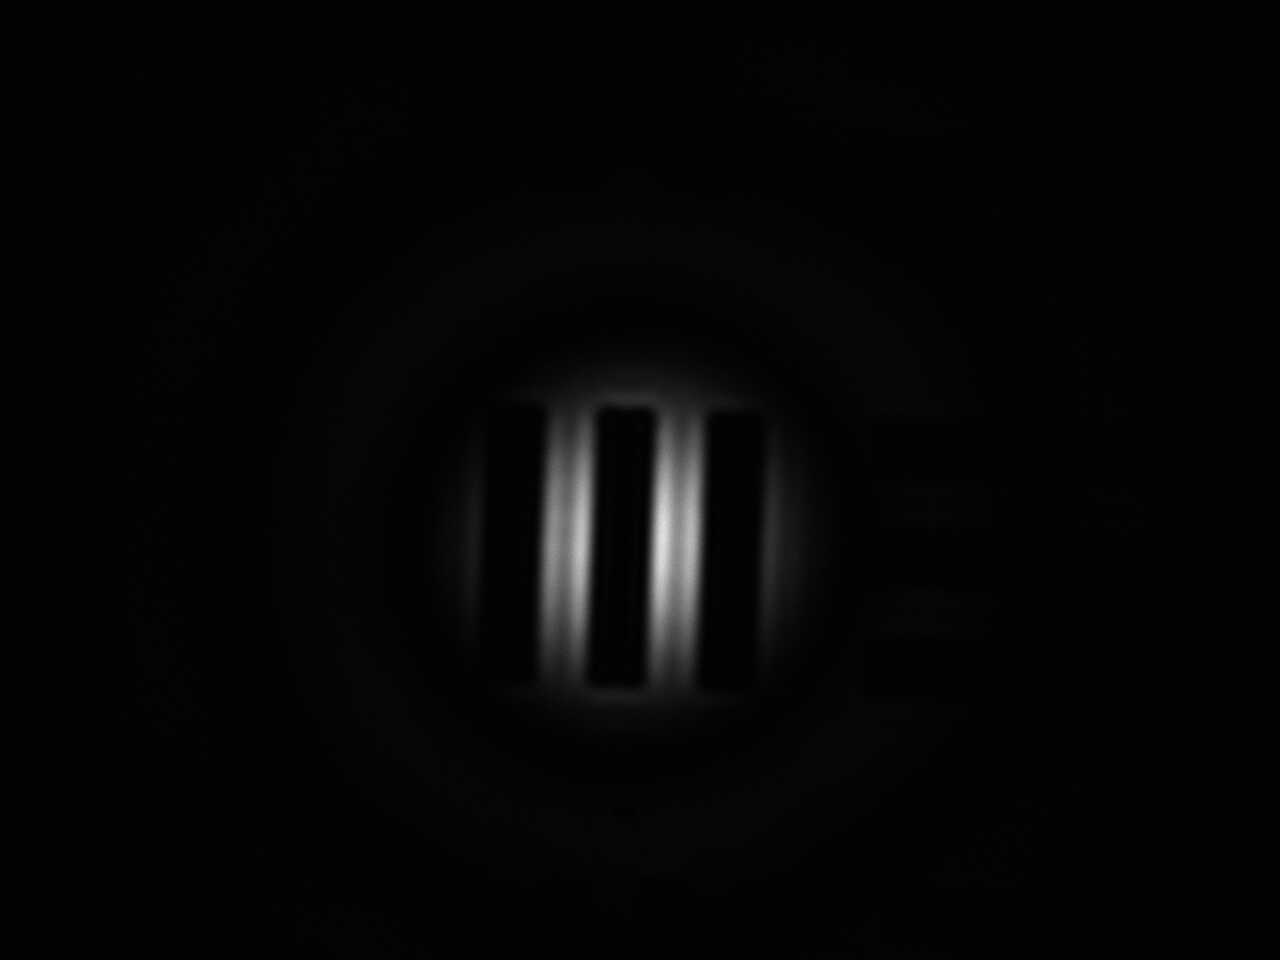
\includegraphics[scale=0.1]{jw/L_OB_3.jpg}
\caption{Aufnahme des Bildes 3. Ordnung. Aufnahme wurde zur Verfügung gestellt.}\label{fig:bild_3_jw}
\end{figure}
\end{minipage}






\begin{minipage}[t]{.45\textwidth}
\begin{figure}[H]
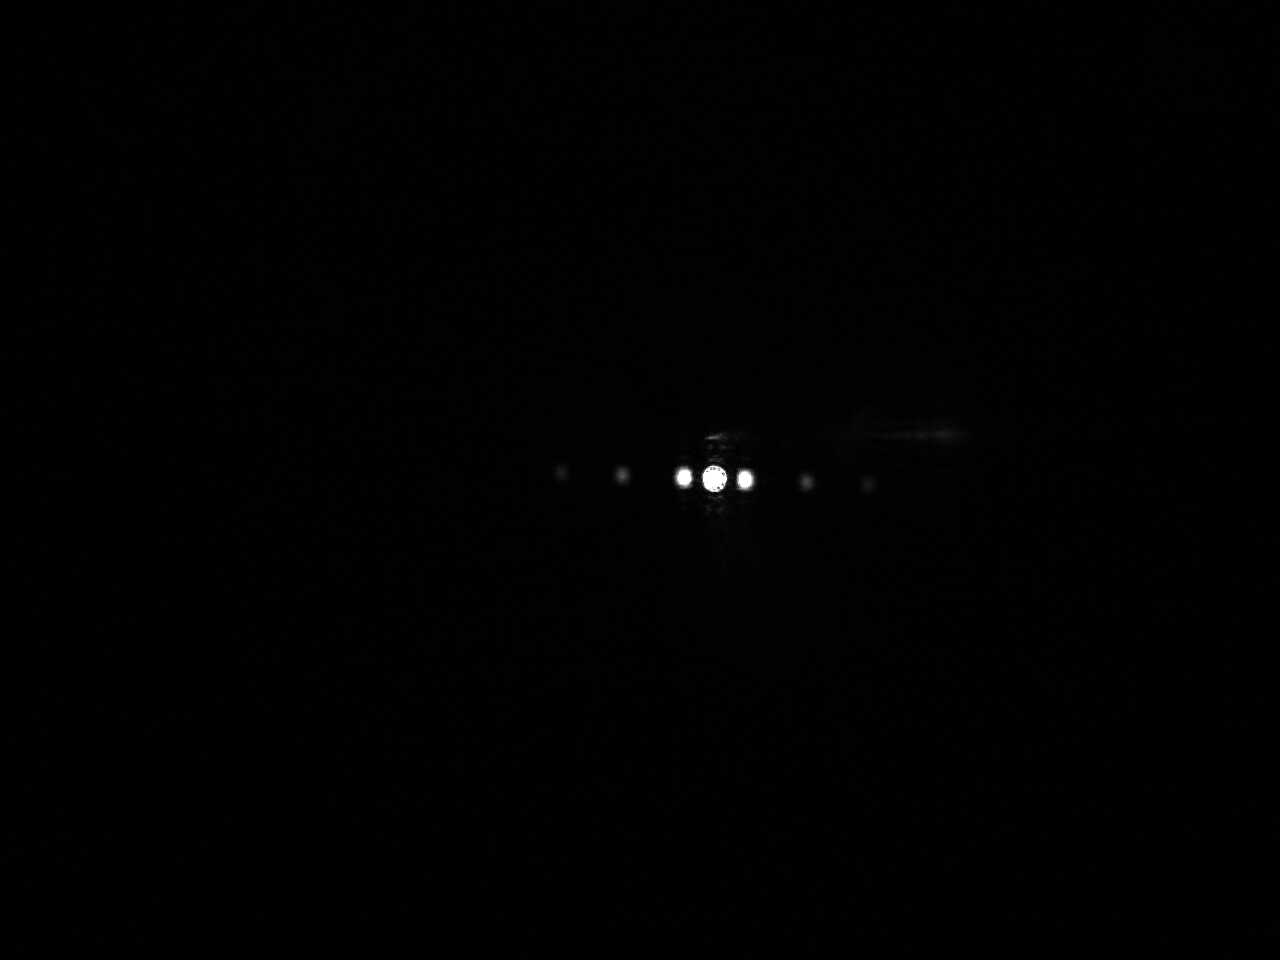
\includegraphics[scale=0.1]{jw/L_BB_2.jpg}
\caption{Aufnahme des Beugungsbildes 5. Ordnung. Aufnahme wurde zur Verfügung gestellt.}
\label{fig:bbild_5_jw}
\end{figure}
\end{minipage}
\hfill
\noindent
\begin{minipage}[t]{.45\textwidth}
\begin{figure}[H]

\includegraphics[scale=0.1]{jw/L_OB_2.jpg}
\caption{Aufnahme des Bildes 5. Ordnung. Aufnahme wurde zur Verfügung gestellt.}\label{fig:bild_5_jw}
\end{figure}
\end{minipage}






\begin{minipage}[t]{.45\textwidth}
\begin{figure}[H]
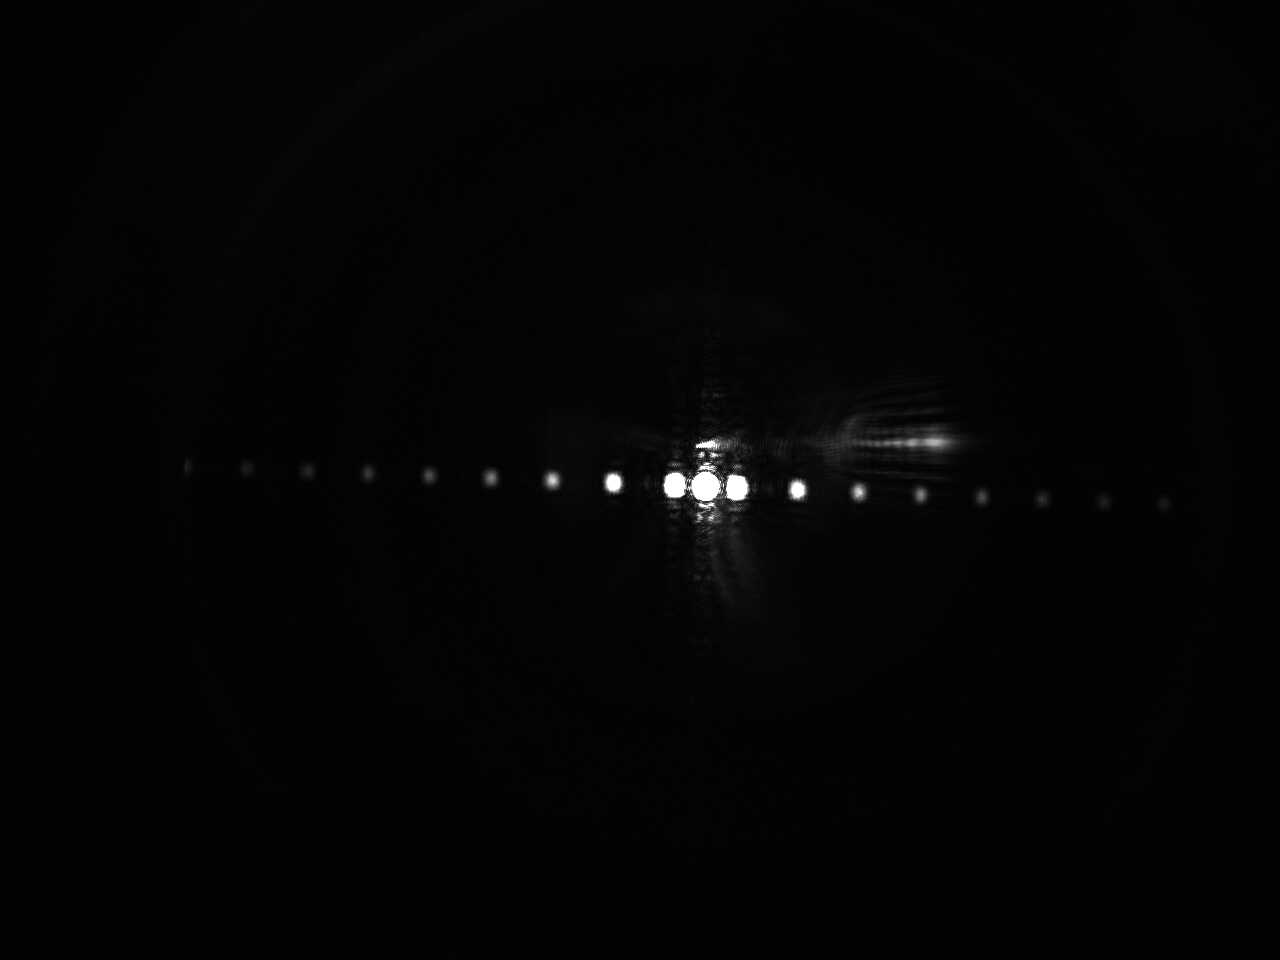
\includegraphics[scale=0.1]{jw/L_BB_1.jpg}
\caption{Aufnahme des Beugungsbildes mit vollständig offener Irisblende. Aufnahme wurde zur Verfügung gestellt.}
\label{fig:bbild_voll_jw}
\end{figure}
\end{minipage}
\hfill
\noindent
\begin{minipage}[t]{.45\textwidth}
\begin{figure}[H]

\includegraphics[scale=0.1]{jw/L_OB_1.jpg}
\caption{Aufnahme des Objektbildes mit vollständig offener Irisblende. Aufnahme wurde zur Verfügung gestellt.}\label{fig:bild_voll_jw}
\end{figure}
\end{minipage}











\newpage


\subsection{Auflösevermögen und Numerische Apertur}



Hier wurden beide LEDs (blau und rot) als Lichtquellen verwendet und die numerische Apertur mit 3 Lochblenden mit verschiedenen Durchmessern variiert. Dann wurden jene Elemente gesucht, bei denen die horizontalen und vertikalen Balken nicht mehr unterscheidbar sind. Von den gefundenen Elementen wurden wieder die Bilder aufgenommen, sowie die eingestellten Lochblenden und die Farbe der LED-Lampe notiert. 

Die von Tanja Maier aufgenommenen Bilder sind in Abbildungen~\ref{fig:bbild_2_blau_tm} bis \ref{fig:bbild_6_rot_tm} gelistet. Die Bilder von Johannes Winkler sind durch die im Moodle gegebenen Aufnahmen ersetzt. Diese wären Abbildungen~\ref{fig:bbild_2_blau_jw} bis \ref{fig:bbild_6_rot_jw}.

\newpage 
\subsubsection{Bilder aufgenommen von Tanja Maier}
\begin{minipage}[t]{.45\textwidth}
\begin{figure}[H]
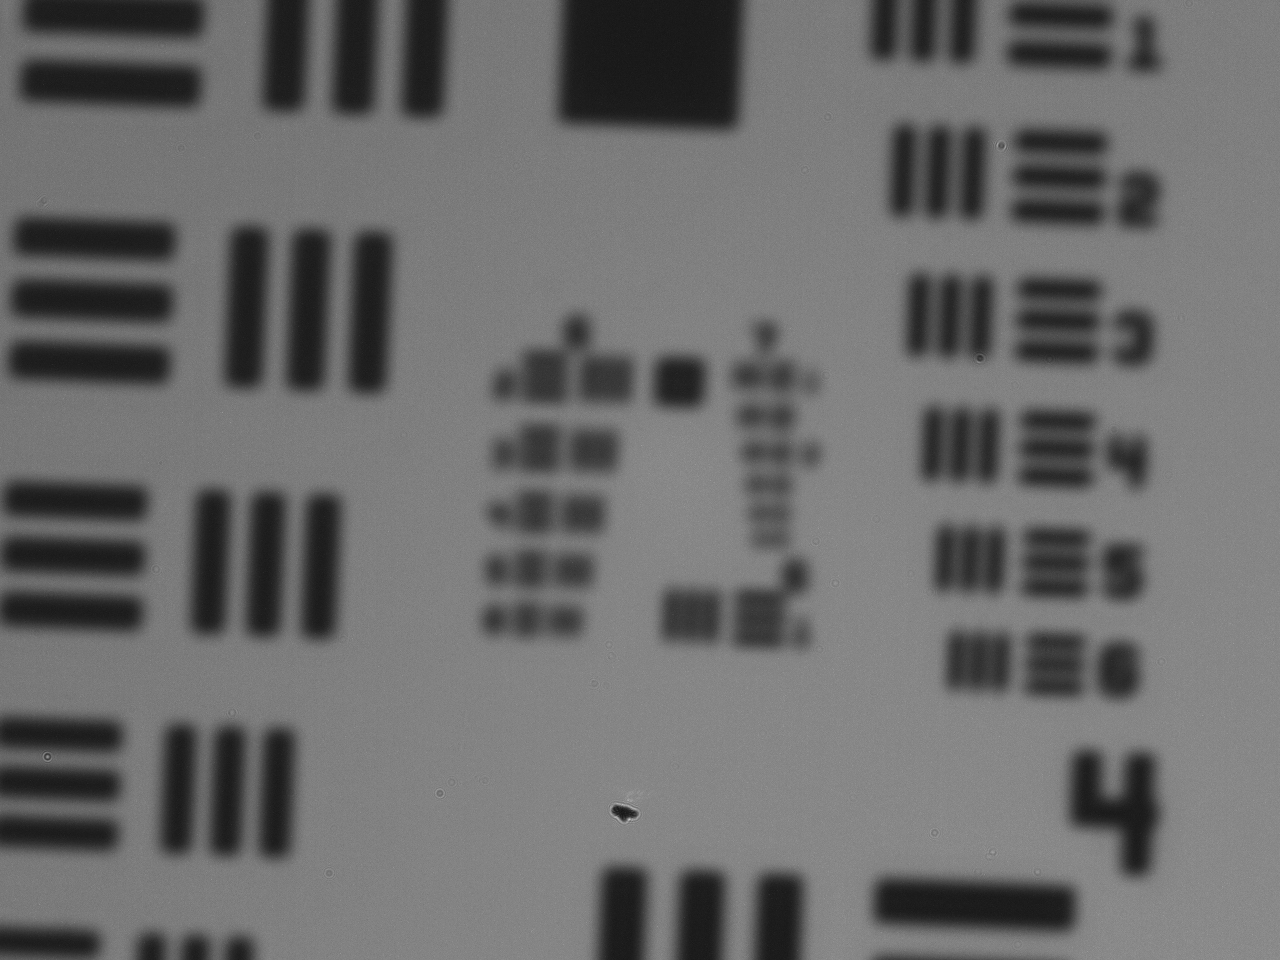
\includegraphics[scale=0.5]{tm/Bild_blau_kleine Lochblende.jpg}
\caption{Beleuchtung mit blauem LED mit einem Blendendurchmesser $d_1=(2.0\pm0.1)~$mm.}
\label{fig:bbild_2_blau_tm}
\end{figure}
\end{minipage}
\hfill
\noindent
\begin{minipage}[t]{.45\textwidth}
\begin{figure}[H]
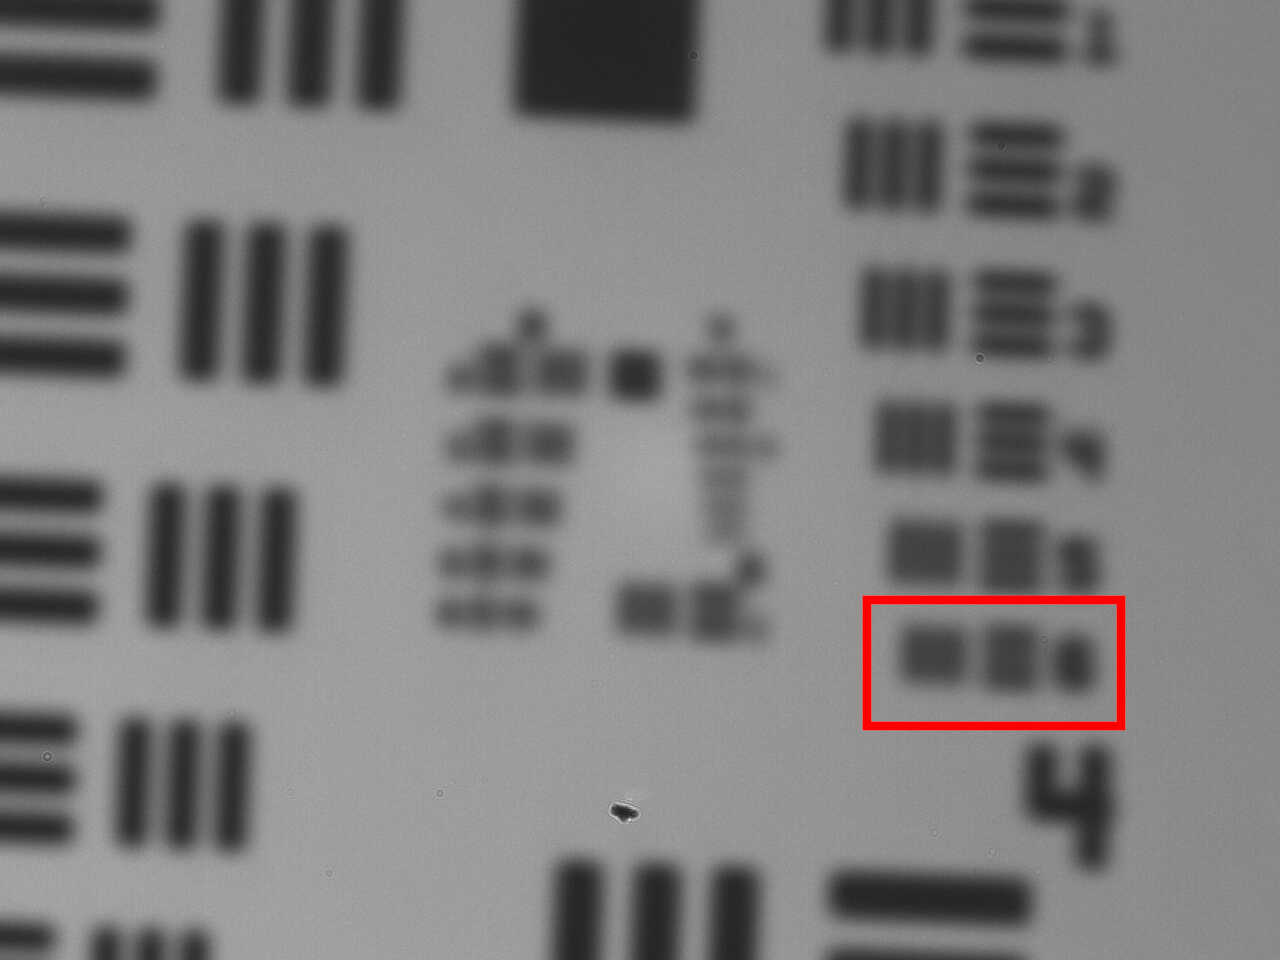
\includegraphics[scale=0.5]{tm/Bild_rot_kleine Lochblende.jpg}
\caption{Beleuchtung mit rotem LED mit einem Blendendurchmesser $d_1=(2.0\pm0.1)~$mm.}
\label{fig:bbild_2_rot_tm}
\end{figure}
\end{minipage}



\begin{minipage}[t]{.45\textwidth}
\begin{figure}[H]
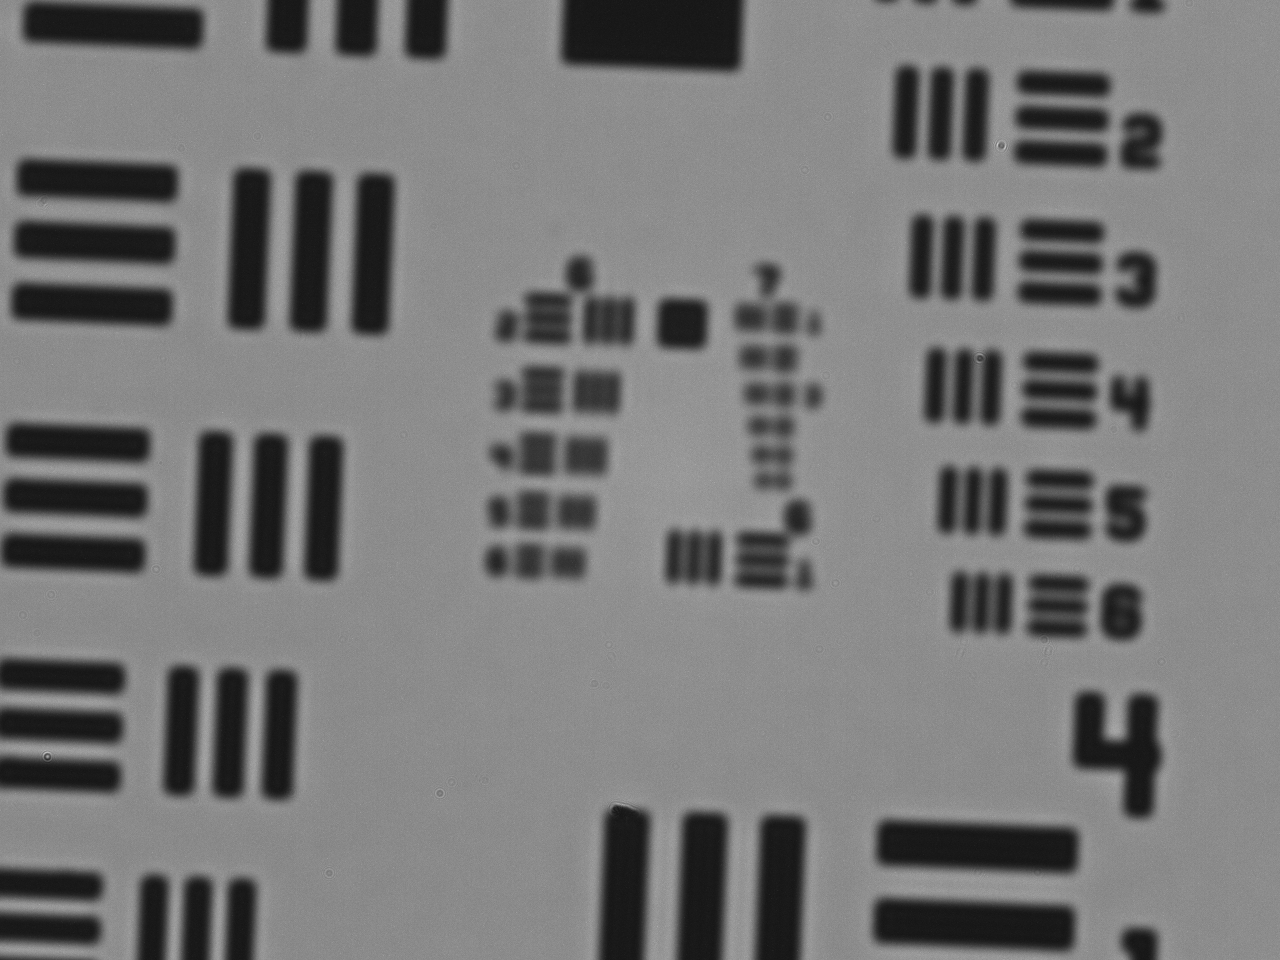
\includegraphics[scale=0.5]{tm/Bild_blau_mittlere Lochblende.jpg}
\caption{Beleuchtung mit blauem LED mit einem Blendendurchmesser $d_2=(3.0\pm0.1)~$mm.}
\label{fig:bbild_3_blau_tm}
\end{figure}
\end{minipage}
\hfill
\noindent
\begin{minipage}[t]{.45\textwidth}
\begin{figure}[H]
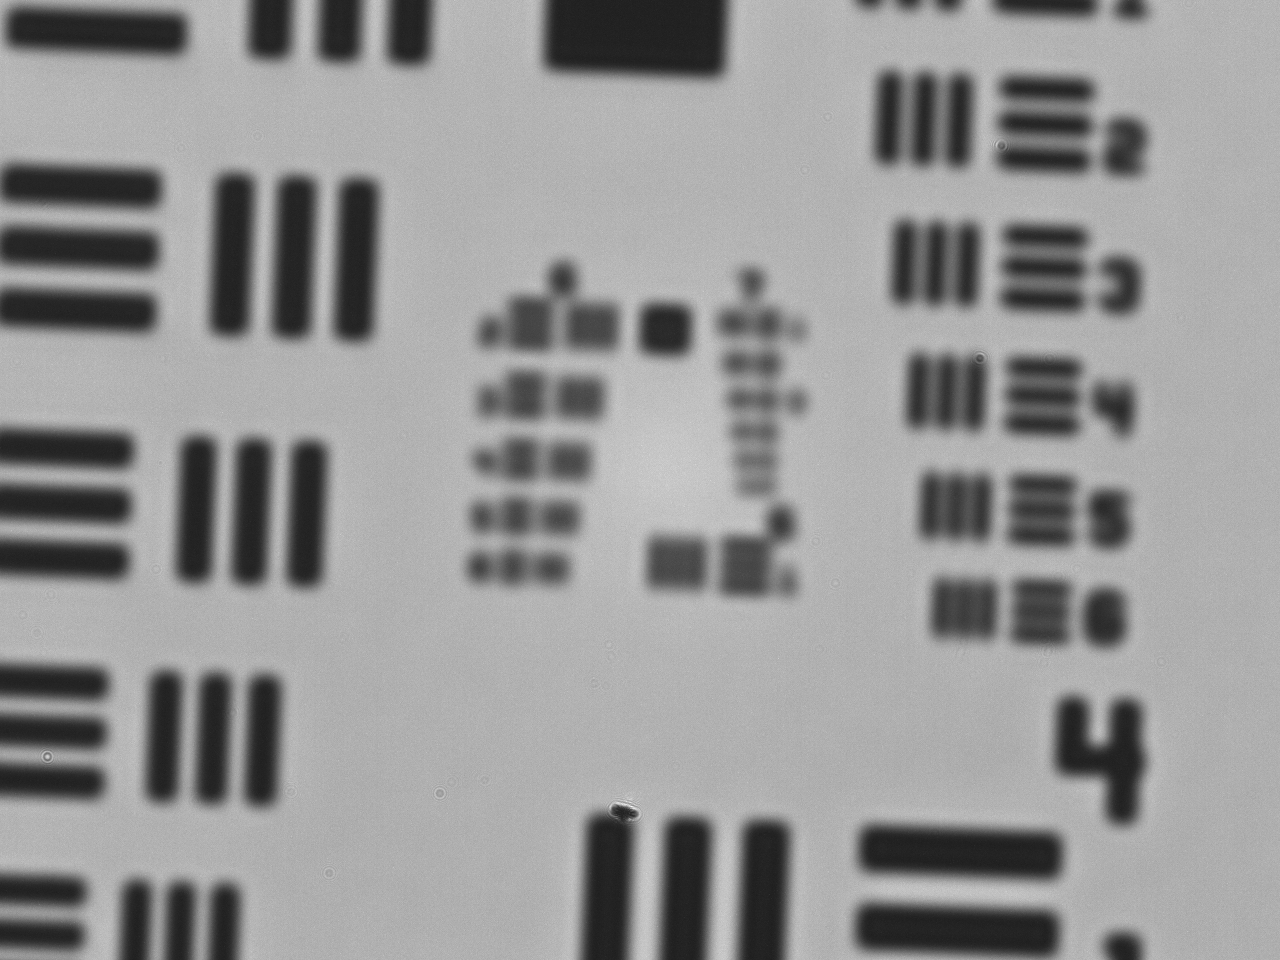
\includegraphics[scale=0.5]{tm/Bild_rot_mittlere Lochblende.jpg}
\caption{Beleuchtung mit rotem LED mit einem Blendendurchmesser $d_2=(3.0\pm0.1)~$mm.}
\label{fig:bbild_3_rot_tm}
\end{figure}
\end{minipage}




\begin{minipage}[t]{.45\textwidth}
\begin{figure}[H]
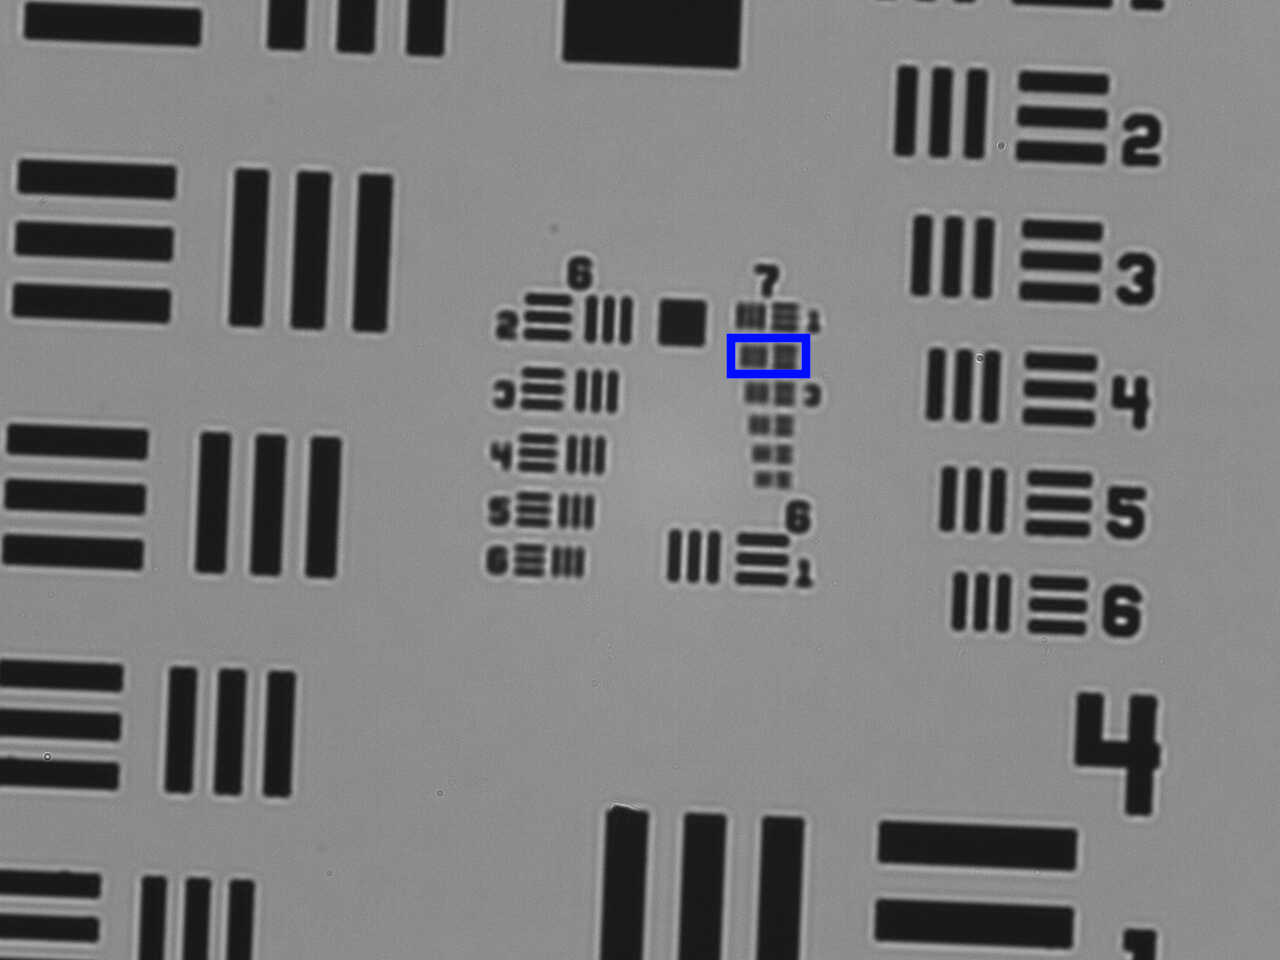
\includegraphics[scale=0.5]{tm/Bild_blau_grosse Lochblende.jpg}
\caption{Beleuchtung mit blauem LED mit einem Blendendurchmesser $d_3=(6.0\pm0.1)~$mm.}
\label{fig:bbild_6_blau_tm}
\end{figure}
\end{minipage}
\hfill
\noindent
\begin{minipage}[t]{.45\textwidth}
\begin{figure}[H]
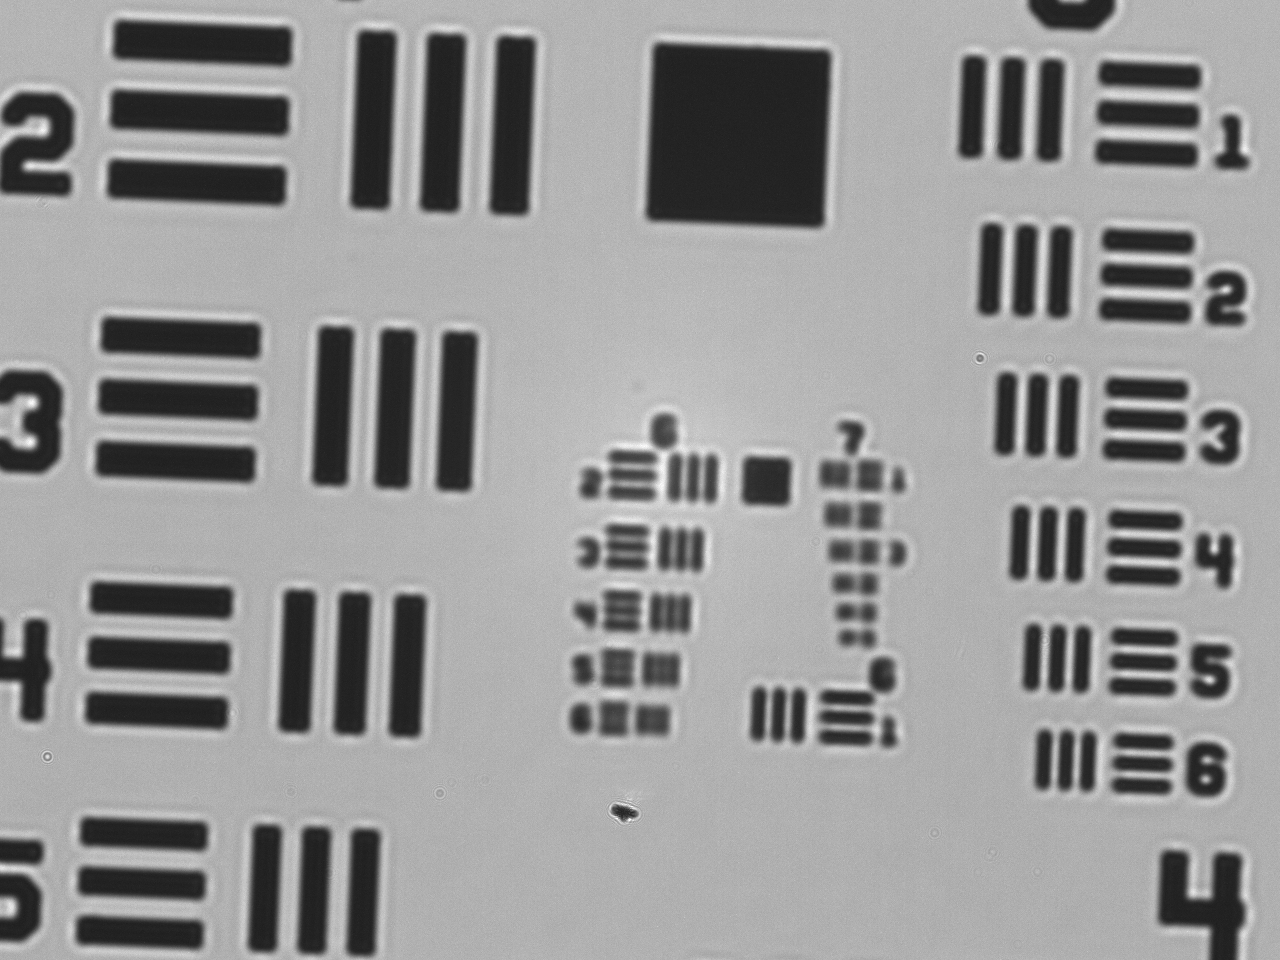
\includegraphics[scale=0.5]{tm/Bild_rot_grosse Lochblende.jpg}
\caption{Beleuchtung mit rotem LED mit einem Blendendurchmesser $d_3=(6.0\pm0.1)~$mm.}
\label{fig:bbild_6_rot_tm}
\end{figure}
\end{minipage}


\newpage




\subsubsection{Bilder aus Mitschrift von Moodle entnommen}


\begin{minipage}[t]{.45\textwidth}
\begin{figure}[H]
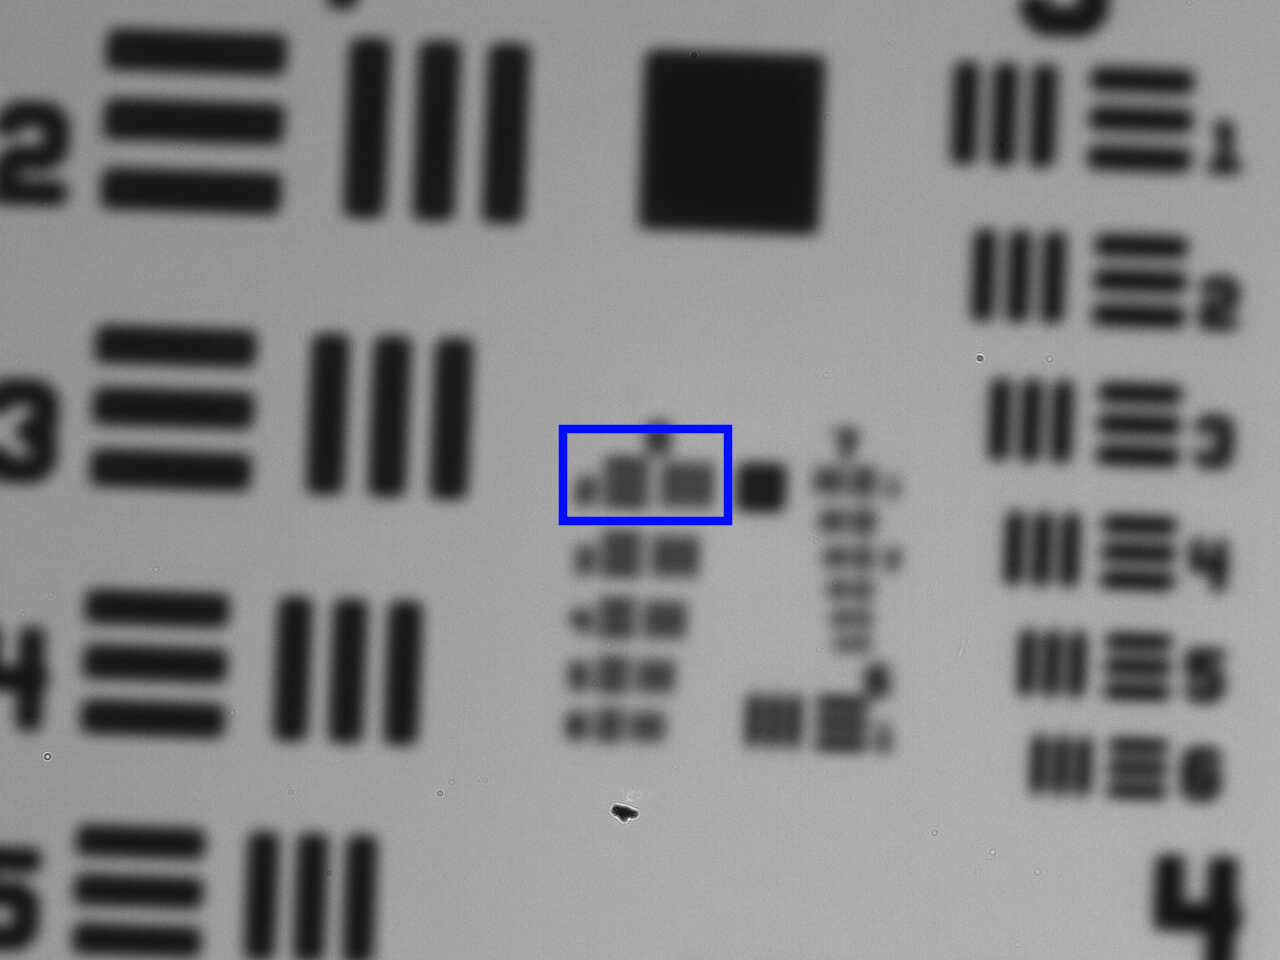
\includegraphics[scale=0.5]{jw/B_B2_mark.jpg}
\caption{Beleuchtung mit blauem LED mit einem Blendendurchmesser $d_1=(2.0\pm0.1)~$mm.}
\label{fig:bbild_2_blau_jw}
\end{figure}
\end{minipage}
\hfill
\noindent
\begin{minipage}[t]{.45\textwidth}
\begin{figure}[H]
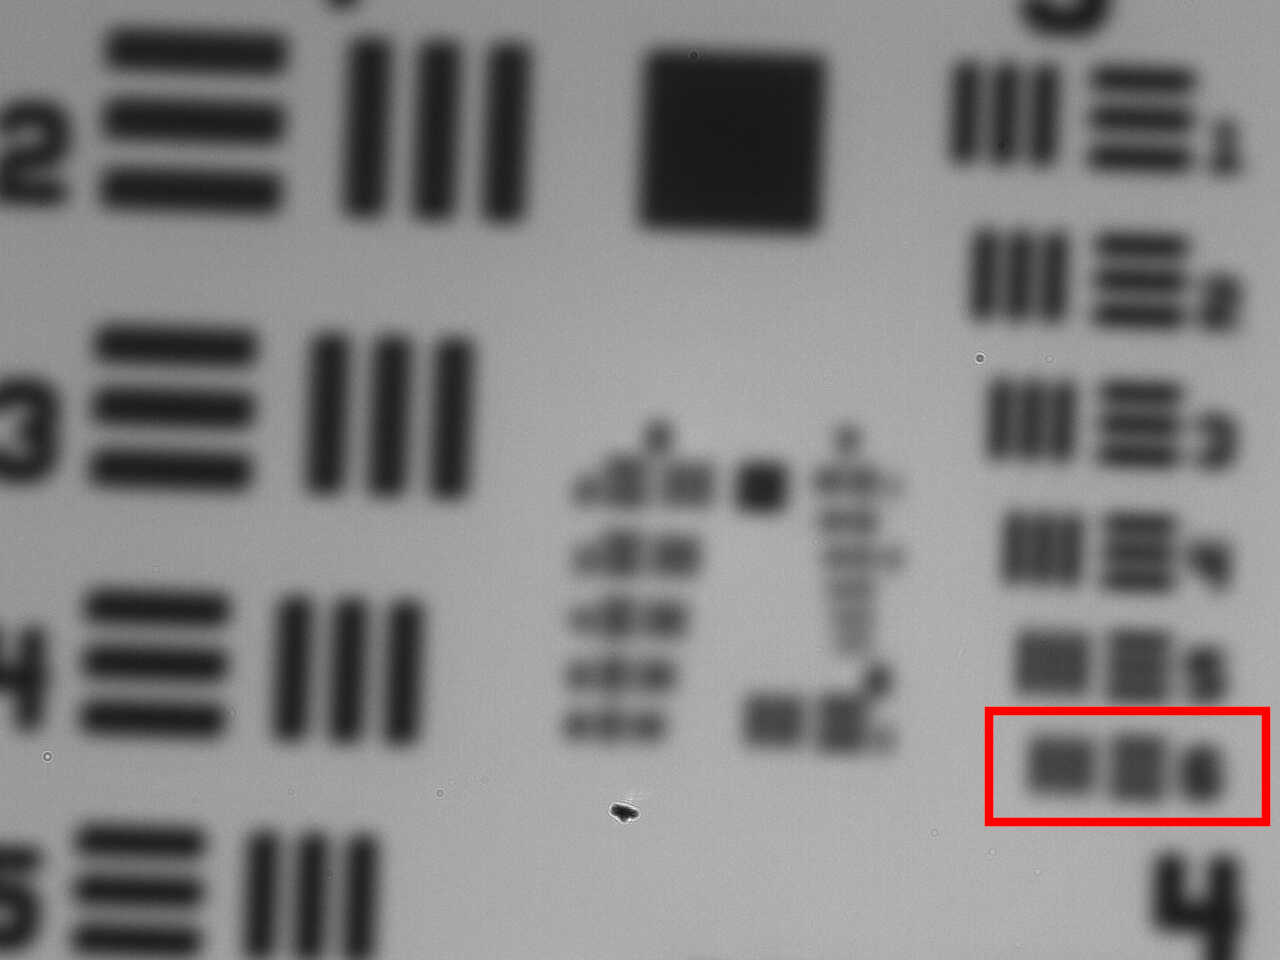
\includegraphics[scale=0.5]{jw/R_B2_mark.jpg}
\caption{Beleuchtung mit rotem LED mit einem Blendendurchmesser $d_1=(2.0\pm0.1)~$mm.}
\label{fig:bbild_2_rot_jw}
\end{figure}
\end{minipage}


\begin{minipage}[t]{.45\textwidth}
\begin{figure}[H]
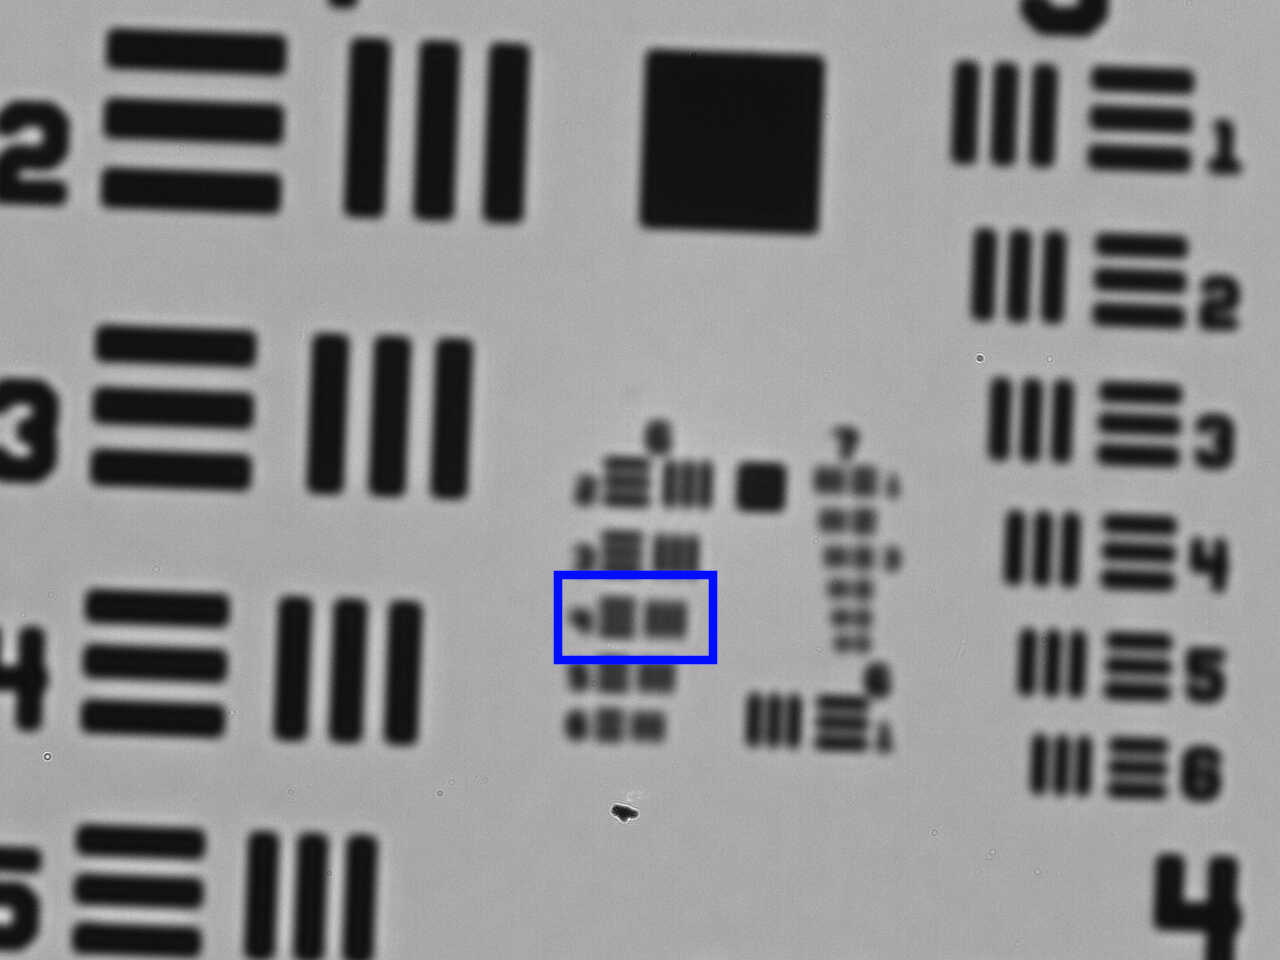
\includegraphics[scale=0.5]{jw/B_B3_mark.jpg}
\caption{Beleuchtung mit blauem LED mit einem Blendendurchmesser $d_2=(3.0\pm0.1)~$mm.}
\label{fig:bbild_3_blau_jw}
\end{figure}
\end{minipage}
\hfill
\noindent
\begin{minipage}[t]{.45\textwidth}
\begin{figure}[H]
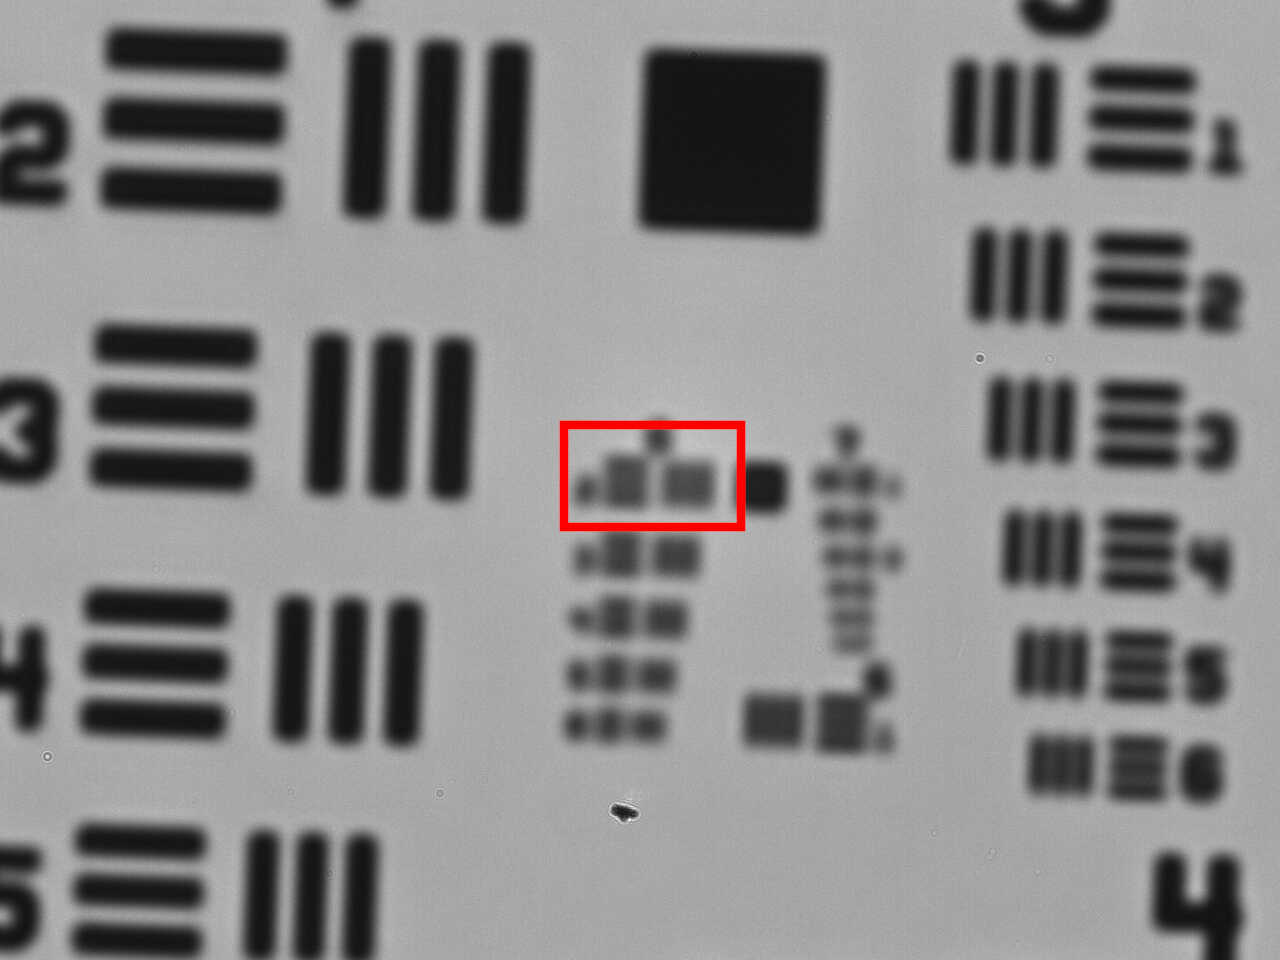
\includegraphics[scale=0.5]{jw/R_B3_mark.jpg}
\caption{Beleuchtung mit rotem LED mit einem Blendendurchmesser $d_2=(3.0\pm0.1)~$mm.}
\label{fig:bbild_3_rot_jw}
\end{figure}
\end{minipage}


\begin{minipage}[t]{.45\textwidth}
\begin{figure}[H]
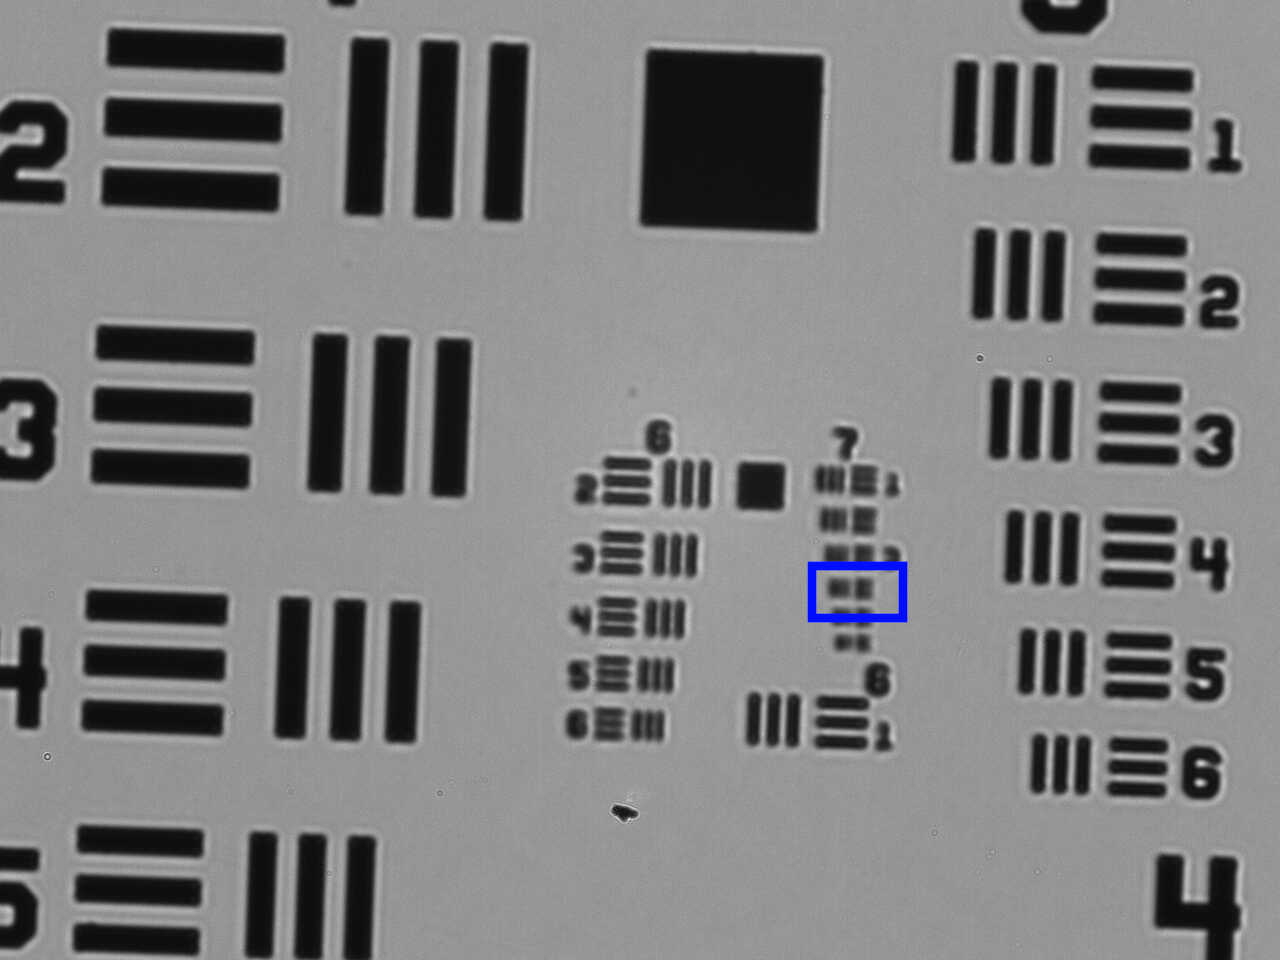
\includegraphics[scale=0.5]{jw/B_B6_mark.jpg}
\caption{Beleuchtung mit blauem LED mit einem Blendendurchmesser $d_3=(6.0\pm0.1)~$mm.}
\label{fig:bbild_6_blau_jw}
\end{figure}
\end{minipage}
\hfill
\noindent
\begin{minipage}[t]{.45\textwidth}
\begin{figure}[H]
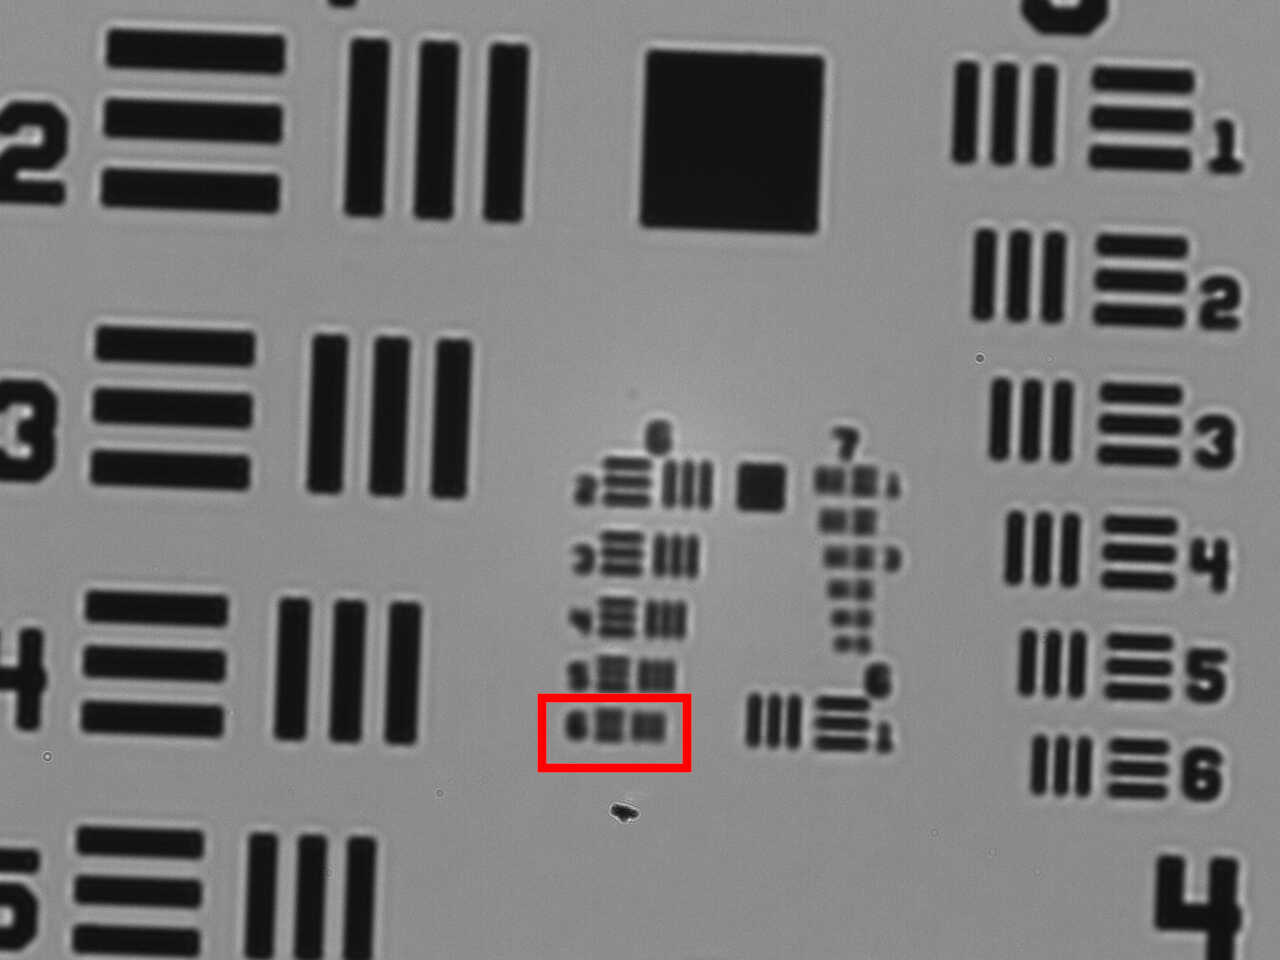
\includegraphics[scale=0.5]{jw/R_B6_mark.jpg}
\caption{Beleuchtung mit rotem LED mit einem Blendendurchmesser $d_3=(6.0\pm0.1)~$mm.}
\label{fig:bbild_6_rot_jw}
\end{figure}
\end{minipage}








\newpage



\section{Auswertung}

\subsection{Beugungsordnungen und Auflösung}

Dieser Versuch läuft qualitativ ab. Hierbei zeigt sich in der Abbe-Theorie, dass in der 0. Beugungsordnung keine Information über die Struktur des Bildes übertragen wird. Um eine genauere Struktur zu erhalten, benötigt man also höhere Begungsordnungen.




\subsection{Auflösevermögen und Numerische Apertur}


Nach Gleichung~\eqref{eq:na} wird zuerst die numerische Apertur berechnet.
\begin{align*}
N_A \approx \frac{d}{2\cdot f} \pm \frac{1}{2}\cdot \left( \frac{\Delta d\cdot f +  d\cdot \Delta f}{f^2}\right)
\end{align*}
wobei $f=f_2$ die Brennweite von L2 ist. Gemäß Geräteliste gilt $f = (60\pm1)~$mm und $\Delta d =  0.01~$mm.


\begin{table}[H]
\caption{Berechnung der numerische Apertur $N_A$. berechnet mit Gleichung~\eqref{eq:na} mit $f=(60\pm1)~$mm. $d$ Durchmesser (Blende), $\Delta d = \pm 0.1$~mm,}
\label{tab:na}
\begin{tabular}{ll}
$d$ / mm  & $N_A$ / 1 \\
\hline
2 & $(16.7 \pm 1.1)\cdot 10^{-3}$ \\
3 & $(25.0 \pm 1.3)\cdot 10^{-3}$ \\
6 & $(50.0 \pm 1.7)\cdot 10^{-3}$
\end{tabular}
\end{table}





\begin{table}[H]
\caption{Gefundene Elemente des 1951 USAF Targets, wo sich die Längs- und Querstreifen nicht mehr unterscheiden lassen. Einmal für die Messungen von Tanja Maier, einmal von den Messergebnissen aus Moodle. $d$ Durchmesser (Blende), $E_b$ bzw. $E_r$ in Versuch 2 gefundenes Element für blaues bzw. rotes Licht.}

\begin{tabular}{l|rr|rr}
& \multicolumn{2}{p{2.5cm}|}{Werte von  ~~ Tanja Maier} & \multicolumn{2}{p{2.5cm}}{Werte von Labor\-mitschrift} \\
$d$ / mm  & $E_b$ & $E_r$ & $E_b$ & $E_r$   \\
\hline
2 &  6/1 & 5/6 & 6/1 & 5/6 \\
3 &  6/4 & 6/1 & 6/4 & 6/1 \\
6 &  7/2 & 6/6 & 7/4 & 6/6
\end{tabular}
\end{table}


Man kann dann die theoretische Auflösung mit der gemessenen Auflösung vergleichen. Die theoretische Auflösung $d_{\text{theor}}$ erhält man durch Formel~\eqref{eq:theor_aufl}. Die theoretischen Auflösungen sind auch in Tabelle~\ref{tab:theor_aufl} aufgelistet.


\begin{table}[H]
\caption{Theoretische Auflösungen $d_\text{theor}$ in Abhängigkeit der numerische Apertur $N_A$ berechnet mit Gleichung~\eqref{eq:theor_aufl}. Berechnung jeweils für rotes und blaues Licht der gegebenen Wellenlängen.}
\label{tab:theor_aufl}
\begin{tabular}{l|l|rr}
$d$ / mm  & $N_A$ / 1 & $d_\text{theor,blau}$ / $\mu$m & $d_\text{theor,rot}$ / $\mu$m\\
\hline
2 & $(16.7 \pm 1.1)\cdot 10^{-3}$ & $17.2 \pm 1.3$ & $23.2 \pm 1.7$ \\
3 & $(25.0 \pm 1.3)\cdot 10^{-3}$ & $11.5 \pm 0.7$ & $15.5 \pm 0.9$ \\
6 & $(50.0 \pm 1.7)\cdot 10^{-3}$ & $5.7 \pm 0.3$ & $7.7 \pm 0.3$ 
\end{tabular}
\end{table}

Die theoretischen Auflösungen in Abhängigkeit von der numerischen Apertur werden auch für die Kurven in Grafik~\ref{fig:kurven} verwendet, die Auflösung und numerische Apertur für eine bestimmte Wellenlänge verknüpft.

Die gemessenen Auflösungen ergeben sich aus Tabelle~\ref{tab:aufl}. Dort kann für jedes Element $E_b$ und $E_r$ die räumliche Frequenz gesucht werden. Der dazugehörige Kehrwert ist die gemessene Auflösung. Die gemessenen Werte für die Auflösung sind in Tabelle~\ref{tab:gem_aufl} zu sehen.

\begin{table}[H]
\caption{Gemessene Auflösungen für blaues und rotes Licht bei dem jeweiligen Durchmesser $d$ der Blende. $d_{\text{gem,blau}}$ bzw. $d_{\text{gem,rot}}$. Zusätzliche Aufteilungen in Messergebnisse von Tanja Maier und den Werten aus Moodle.}
\label{tab:gem_aufl}

\begin{tabular}{l|rr|rr}
& \multicolumn{2}{p{2.5cm}|}{Werte von  ~~ Tanja Maier} & \multicolumn{2}{p{2.5cm}}{Werte von Labor\-mitschrift} \\
$d$ / mm  & $d_{\text{gem,blau}}$ / $\mu$m & $d_{\text{gem,rot}}$ / $\mu$m & $d_{\text{gem,blau}}$ / $\mu$m & $d_{\text{gem,rot}}$ / $\mu$m   \\
\hline
2 &  $15.6\pm1.8$ & $17.5\pm2.0$ & $15.6\pm1.8$ & $17.5\pm2.0$ \\
3 &  $11.0\pm1.3$ & $15.6\pm1.8$ & $11.0\pm1.3$ & $15.6\pm1.8$ \\
6 &  $6.9\pm0.8$ & $8.8\pm1.0$ & $5.5\pm0.6$ & $8.8\pm1.0$
\end{tabular}
\end{table}







\begin{figure}[H]
\caption{Kurven für die theoretische Auflösung in Abhängigkeit von der numerischen Apertur. Die berechneten Werte für die Auflösung sind zusätzlich eingezeichnet. Ein Ausreisser bei einer numerischen Apertur von 0.05 wrude entsprechend markiert.}
\label{fig:kurven}
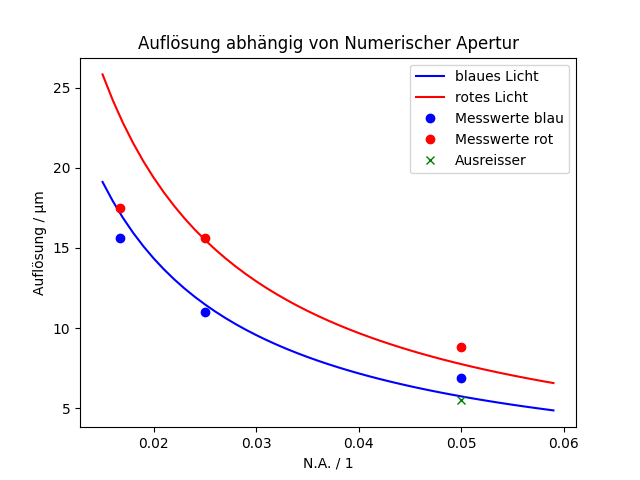
\includegraphics[scale=0.7]{plot.png}

\end{figure}




\section{Zusammenfassung und Diskussion}

Es zeigt sich hier deutlich, dass ein Zusammenhang zwischen der Schärfe des Bildes und der Anzahl der Beugungsordnungen gilt. Und zwar wird das Bild mit der Anzahl der verwendeten Beugungsordnungen schärfer. Damit kann die Abbe Theorie experimentell verifiziert werden.

~

Im zweiten Teil zeigt sich, dass das Bild bei blauem LED höher aufgelöst (also $d$ kleiner) ist. Dies liegt an der kürzeren Wellenlänge von blauem Licht. Zwischen den Messwerten von Tanja Maier und den zur Verfügung gestellten Messwerten aus Moodle gab es im wesentlichen einen Unterschied beim Blendendurchmesser von 6~mm. Während der von Tanja Maier gemessene Wert 6.9~$\mu$m beträgt, ergab der Wert aus Moodle 5.5~$\mu$m. Tendenziell sieht man, dass bei höheren Auflösungen (kleineren Wertern für $d$) die Abweichung von den theoretischen Werten kleiner ist. Die Ursache dafür könnten Ablesefehler sein.






%\newpage 
%\appendix
%\section{Python Skript}



\definecolor{commentgreen}{RGB}{2,112,10}
\definecolor{eminence}{RGB}{108,48,130}
\definecolor{weborange}{RGB}{255,165,0}
\definecolor{frenchplum}{RGB}{129,20,83}

\lstdefinelanguage{python}{
    morekeywords={def, for, range, abs, return},
    otherkeywords={<-,->, |>, \%\{, \}, \{, \, (, )},
    sensitive=true,
    morecomment=[l]{\#},
    morecomment=[n]{/*}{*/},
    morecomment=[s][\color{purple}]{:}{\ },
    morestring=[s][\color{orange}]"",
    commentstyle=\color{commentgreen},
    keywordstyle=\color{eminence},
    stringstyle=\color{red},
	basicstyle=\ttfamily,
	breaklines,
	showstringspaces=false,
	frame=tb
}
%\lstinputlisting[language=Python,captionpos=b, label=lst:test,caption={Python Skript}]{generate_numbers.py}

%\lstinputlisting[language=Python,captionpos=b, label=lst:test,caption={Bessel Auswertung}]{generate_numbers_bessel.py}


%\lstinputlisting[language=Python,captionpos=b, label=lst:test,caption={Zerstreuungslinse Auswertung}]{generate_numbers_zerstreuungslinse.py}


\begin{thebibliography}{9}
\bibitem{quelle1} \url{https://www.youtube.com/watch?v=oFJCEGcwUiQ}, 07.11.2020, 00:15 Uhr
\bibitem{quelle2} \url{https://www.spektrum.de/lexikon/physik/abbesche-theorie/13}, 07.11.2020, 00:17 Uhr
\bibitem{quelle3} \url{https://www.univie.ac.at/mikroskopie/1_grundlagen/optik/opt_instrumente/7_abbe.htm}, 07.11.2020, 00:24 Uhr
\bibitem{quelle4} \url{https://physik.cosmos-indirekt.de/Physik-Schule/Rayleigh-Kriterium}, 07.11.2020, 00:26 Uhr
\bibitem{quelle5} \url{https://www.youtube.com/watch?v=PZaUY45ce8k}, 07.11.2020, 00:27 Uhr
\bibitem{quelle6} Unterlagen aus Moodle, H. Ditlbacher, bereitgestellt von der KF Universität Graz
\bibitem{demtroeder} W. Demtröder: \emph{Experimentalphysik 2 - Elektrizität  und Optik}, 7. Auflage, 2017.
\end{thebibliography}


\end{document}
